\documentclass{elsarticle}
\usepackage{hyperref}
\usepackage[utf8]{inputenc}
\usepackage{wrapfig}
\usepackage{amsmath}
\usepackage{amsthm}
\usepackage{amssymb}
\usepackage[tmargin=1in,bmargin=1in]{geometry}
\usepackage{caption}
\usepackage{graphicx}
\usepackage{latexsym}
\usepackage{pdfsync}
\usepackage[boxed]{algorithm}
\usepackage{algorithm}
%\usepackage{algpseudocode}
\usepackage{multirow}
\usepackage{rotating}
\usepackage{color}
\usepackage{url}
\usepackage{subfigure}
\usepackage{bigstrut}
\usepackage{bigints}
\usepackage[normalem]{ulem}

\usepackage[normalem]{ulem}




\hypersetup{
    colorlinks=true,              % false: boxed links; true: colored links
    linkcolor=blue,               % color of internal links
    citecolor=blue,               % color of links to bibliography
    filecolor=black,              % color of file links
    urlcolor=red,               % color of external links
    bookmarks=false,
    pdffitwindow=true,
    pdfpagelayout=SinglePage
}

\captionsetup[figure]{font=small,labelfont=normal}

\definecolor{mypink}{cmyk}{0, 0.7808, 0.4429, 0.1412}

\definecolor{mybrown}{cmyk}{0, 0.60, 0.95, 0.63}
\definecolor{darkgreen}{cmyk}{0.98, 0, 0.36, 0.22}


\newcommand{\comment}[1]{\textcolor{red}{[#1]$_{\rm Frederic}$}}
\newcommand{\pouriacomment}[1]{\textcolor{darkgreen}{[#1]$_{\rm Pouria}$}}

\newcommand{\etal}{\textit{et al.\ }}
\newcommand{\pd}[2]{\frac{\partial #1}{\partial #2}}
\newcommand{\mbf}[1]{\mathbf{#1}}
\newcommand{\vect}[1]{\boldsymbol{#1}}
\newcommand{\tensor}[1]{\underline{\underline{\boldsymbol{#1}}}}
\newcommand{\mat}[1]{\underline{\underline{\boldsymbol{#1}}}}
\newcommand{\be}{\begin{equation}}
\newcommand{\ee}{\end{equation}}
\newcommand{\ben}{\begin{equation*}}
\newcommand{\een}{\end{equation*}}
\newcommand{\bea}{\begin{eqnarray}}
\newcommand{\eea}{\end{eqnarray}}
\newcommand{\bean}{\begin{eqnarray*}}
\newcommand{\eean}{\end{eqnarray*}}

\newcommand{\fphi}[2]{\frac{\phi_#1}{\phi_#1-\phi_#2}}
\newcommand{\lif}[2]{\frac{f_#1\phi_#2-f_#2\phi_#1}{\phi_#2-\phi_#1}}
\newcommand{\dx}{{\Delta x}}
\newcommand{\dy}{{\Delta y}}
\newcommand{\dz}{{\Delta z}}
\newcommand{\dt}{{\Delta t}}
\newcommand{\hf}{{\frac12}}
\newcommand{\U}{\vect{U}}
\newcommand{\n}{\vect{n}}



\usepackage{algorithm}
\usepackage[noend]{algpseudocode}
\makeatletter
\def\BState{\State\hskip-\ALG@thistlm}
\makeatother



\begin{document}
%\title{JAX-DIPS: Differentiable Interfacial PDE Solver}
%\title{Differentiable framework for learning surrogate neural network models for solving elliptic problems with discontinuities across irregular interfaces}
%\title{Differentiable residual minimization method for learning surrogate models for elliptic problems with irregular discontinuities}

\title{JAX-DIPS: Neuro-symbolic bootstrapping method for solving elliptic problems with discontinuities across irregular interfaces}

\cortext[cor]{Corresponding author: p.a.mistani@gmail.com}


\author[1]{Pouria A. Mistani\thanks{corresponding author} $^{\dagger,}$}
\author[2]{Samira Pakravan$^{\dagger,}$}
\author[1]{Rajesh Ilango}
\author[2]{Frederic G. Gibou}

\address[1]{NVIDIA Corporation, Santa Clara, CA 95051, USA}
\address[2]{University of California, Santa Barbara, CA 93106-5070, USA}

\begin{abstract}
	We present a scalable strategy for development of mesh-free hybrid neuro-symbolic partial differential equation solvers based on existing mesh-based numerical discretization methods. Particularly, this strategy can be used to efficiently train neural network surrogate models for the solution of partial differential equations while retaining the accuracy and convergence properties of the state-of-the-art numerical solvers. The presented neuro-symbolic bootstrapping method (hereby dubbed NSBM) is based on evaluation of the finite discretization residuals of the PDE system obtained on implicit Cartesian cells centered on a set of random collocation points with respect to trainable parameters of the neural network. We apply NSBM to the challenging class of elliptic problems with jump conditions across irregular sharp interfaces in three spatial dimensions. We show the method is convergent such that model accuracy improves by increasing number of collocation points in the domain.  The algorithms presented here are implemented and released in a software package named \texttt{JAX-DIPS} (\href{https://github.com/JAX-DIPS/JAX-DIPS}{https://github.com/JAX-DIPS/JAX-DIPS}), standing for differentiable interfacial PDE solver. \texttt{JAX-DIPS} is purely developed in \texttt{JAX}, offering end-to-end differentiability from mesh generation to the higher level discretization abstractions, geometric integrations, and interpolations, thus facilitating research into use of differentiable algorithms for developing hybrid PDE solvers.

\end{abstract}

\begin{keyword}
	level-set method \sep free boundary problems \sep surrogate models \sep jump conditions \sep differentiable programming \sep neural networks
\end{keyword}

\maketitle
\def\thefootnote{$\dagger$}\footnotetext{These authors contributed equally to this work}







%%%%%%%%%%%%%%%%%%%%%%%%%%%%%%%%%%%%%
%%%%%%%%%%%%%%%%%%%%%%%%%%%%%%%%%%%%%
\section{Introduction}
\label{sec::introduction}

\subsection{Problem statement}
Consider a closed irregular interface ($\rm \Gamma$) that partitions the computational domain ($\rm \Omega$) into interior ($\rm \Omega^-$) and exterior ($\rm \Omega^+$) subdomains; \textit{i.e.}, $\rm \Omega=\Omega^- \cup \Gamma \cup \Omega^+$. We are interested in the solutions $\rm u^\pm\in \Omega^\pm$ to the following class of linear elliptic problems in  $\rm \mathbf{x}\in\Omega^\pm$:
\begin{align*}
	 & k^{\pm}u^{\pm} - \nabla \cdot (\mu^{\pm}\nabla u^\pm)=f^{\pm}, & \mathbf{x}\in\Omega^\pm \\
	 & [u]=\alpha,                                                    & \mathbf{x} \in \Gamma   \\
	 & [\mu \partial_{\mathbf{n}}u]=\beta,                            & \mathbf{x} \in \Gamma
\end{align*}
Here $f^\pm=f(\mathbf{x} \in \Omega^\pm)$ is the spatially varying source term, $\rm \mu^\pm=\mu(\mathbf{x} \in \Omega^\pm)$  are the diffusion coefficients, and $k^\pm$ are the reaction coefficients in the two domains. We consider Dirichlet boundary conditions in a cubic domain $\rm \Omega=[-L/2,L/2]^3$.


This class of problems arise ubiquitously in describing diffusion dominated processes in physical systems and life sciences where sharp and irregular interfaces regulate transport across regions with different properties. Examples include Poisson-Boltzmann equation for describing electrostatic properties of membranes, colloids and solvated biomolecules with jump in dielectric permittivities \cite{sharp1990calculating,MirzadehPB}, electroporation of cell aggregates with nonlinear membrane jump conditions \cite{mistani2019parallel}, epitaxial growth in fabrication of opto-electronic devices where atomic islands grow by surface diffusion of adatoms across freely moving interfaces \cite{MISTANI2018150}, solidification of multicomponent alloys used for manufacturing processes with free interfaces separating different phases of matter \citep{theillard2015sharp,bochkov2021sharp}, directed self-assembly of diblock copolymers for next generation lithography \cite{galatsis2010patterning,ouaknin2018level,bochkov2021non}, multiphase flows with and without phase change, and Poisson-Nernst-Planck equations for electrokinetics. Much of these processes are multiscale and the changes across interfaces must be mathematically modeled and numerically solved as sharp surfaces. Smoothing strategies introduce unphysical characteristics in the solution and lead to systemic errors.

\subsection{Literature on relevant finite discretization methods}
Several numerical methods have been proposed for accurate solution of this class of problems based on explicit or implicit representation of the interface. Finite element methods rely on explicit meshing of the surface that poses severe challenges \cite{babuvska1970finite,bramble1996finite}. Implicit methods include the Immersed Interface Method (IIM) \cite{leveque1994immersed} and its variants \cite{adams2002immersed,li2003new,ewing1999immersed,gong2008immersed} that rely on Taylor expansions of the solution on both sides of the interface and modifying the local stencils to impose the jump conditions. The main challenge is evaluating high order jump conditions and surface derivatives along interface. Another method is the Ghost Fluid Method (GFM) \cite{fedkiw1999non} that was originally introduced to approximate two-phase compressible flows and later applied to the Poisson problem with jump conditions \cite{liu2000boundary}. The basic idea is to define fictitious fluid regions across the discontinuities by adding jump conditions to the true fluid. While GFM captures the normal jump in solution accurately, the tangential jump is smeared. This was solved by the Voronoi Interface Method (VIM) \cite{guittet2015solving} by applying the GFM treatment on a local Voronoi mesh by adapting a local Cartesian mesh which introduces numerical challenges. Several other approaches include the cut-cell method \cite{crockett2011cartesian}, discontinuous Galerkin and eXtended Finite Element Method (XFEM) \cite{lew2008discontinuous,moes1999finite,belytschko2001arbitrary} among others.

In this work we bootstrap the level-set based finite volume method on Cartesian grids proposed by Bochkov \& Gibou (2020) \cite{BOCHKOV2020109269}. This method is based on the idea of Taylor expansions in the normal direction and employing one-sided least-square interpolations for imposing jump conditions. In particular, this method offers second order accurate numerical solutions with first order accurate gradients in the $\rm L^\infty$-norm.


\subsection{Literature on solving PDEs with neural networks}
Since early 1990s, artificial neural networks have been used for solving partial differential equations by (i) mapping the algebraic operations of the discretized PDE systems onto specialized neural network architectures and minimizing the network energy, or (ii) treating the whole neural network as the basic approximation unit whose parameters are adjusted to minimize a specialized error function that includes the differential equation itself with its boundary/initial conditions. 


In the first category, neurons output the discretized solution values over a set number of grid points and minimizing the network energy drives the neuronal values towards the solution of the linear system at the mesh points. In this case, the neural network energy is the residual of the finite discretization method summed over all neurons of the network \cite{lee1990neural}. Although the convergence properties of the finite discretization methods gaurantee and control quality of the obtained solutions, the computational costs grow by increasing resolution and dimensionality. Interestingly, due to regular and sparse structure of the finite discretizations, such locally connected neural network PDE solvers have been implemented on VLSI analog CMOS circuits \cite{gobovic1993design,chua1988cellular,chua1988cellularA}.


The second strategy proposed by Lagaris \textit{et al.} \cite{lagaris1998artificial} relies on the function approximation capabilities of the neural networks. Encoding the solution everywhere in the domain within a neural network offers a mesh-free, compact, and memory efficient surrogate model for the solution function that can be utilized in subsequent inference tasks. This method has recently re-emerged as the physics-informed neural networks (PINNs) \cite{RAISSI2019686} and is widely used. Despite their advantages, these methods lack controllable accuracy and convergence properties of finite discretization methods.

Pursuit of hybrid solvers aims at leveraging the performance gains of neural network inference on modern accelerated hardware with the gauranteed accuracy of finite discretization methods. The hybridization efforts are algorithmic or architectural.

One important algorithmic method is the deep Galerkin method (DGM) \cite{SIRIGNANO20181339} that is a neural network extension of the mesh-free Galerkin method where the solution is represented as a deep neural network rather than a linear combination of basis functions. The mesh-free nature of DGM, that stems from the underlying mesh-free Galerkin method, enables solving problems in higher dimensions by training the neural network model to satisfy the PDE operator and its initial and boundary conditions on a randomly sampled set of points rather than on an exponentially large grid. Although the number of points is huge in higher dimensions, the algorithm can process training on smaller batches of data points sequentially. Besides, second order derivatives in PDEs are calculated by a Monte Carlo method that retain scaling to higher dimensions. 

Architectural hybridization methods come in different flavors. One emerging class involves implementing differentiable finite discretization solvers and embedding them inside neural network architectures to enable end-to-end differentiable gradient based optimizations. These methods are primarily suitable for inverse problems where an unknown field is modeled by the neural network, while the model effect is propagated by the differentiable solver into a measurable residual in the solution space \cite{pakravan2021solving,dal2020data,lu2020extracting}. Another strategy is explicit implementation of the adjoint method to establish the gradient of the loss \cite{berg2017neural}.



\subsection{Our contributions}
In this work we propose a novel algorithm for solving PDEs based on deep neural networks by lifting any existing mesh-based finite discretization method off of its underlying grid and extend it into a mesh-free method that can be applied to high dimensional problems on unstructured random points in an embarrasingly parallel format. We call our method Neuro-Symbolic Bootstrapping Method (NSBM). Bootstrapping is a technique by which a simple computer program activates a more complicated system of programs.



JAX-DIPS Poisson problem solver provides the two sides of $A u =b$ which is obtained after discretization of the governing PDE problem over a uniform 3D grid. Two solution schemes for the forwards problem are possible: (1) using usual iterative methods having left-hand-side and right-hand-side of the PDE discretization, and (2) using autodifferentiation across loss function (difference between lhs and rhs in 2-norm) with respect to a given estimate for the solution vector on the underlying grid $\rm u_{ijk}$. Both approaches focus on minimizing the residual over the grid points
\begin{align*}
	\min_{u_{ijk}} \vert\vert Au -b \vert \vert^2_2
\end{align*}
The first method attempts to span the residual space in an iterative fashion by \textit{estimating} the gradient of the minimizing function, while the second method offered in JAX-DIPS is directly computing the exact gradient of the minimizing function with respect to the current estimate for solution. Therefore, the advantage of this method is fewer iterations and faster convergence specially for irregular geometries where the condition number of the linear system leads to much difficulties that need to be resolved by complex preconditioning and increased number of iterations.



We designed \texttt{JAX-DIPS} as a modular open source library for the research community on the level-set methods for solving interfacial PDE problems. We invite the community to contribute to this library for further development of novel numerical algorithms for solving both forward and inverse interfacial PDE problems.





%\section{Level-set method for free boundary problems}
\section{Dynamic Geometry Representation}
A differentiable solver for free boundary problems requires a rich data structure capable to handle several geometric operations over a given mesh. We understand the mesh as a \textit{topological} relationships between cells that discretize a domain, the geometric information of this discretization as well as the relative configuration of the interfaces with respect to the cells need to be computed. 

In \texttt{JAX-DIPS} we have implemented a uniform grid that supports operations such as interpolations, interface advection, integrations over interfaces as well as in domains. We describe the numerical algorithms used in this section.


\subsection{Interpolation methods}
To support finite discretization methods for the free boundary problems (namely solver, level-set method, and geometric integrations) a widely needed building block is the ability to interpolate field values anywhere inside a grid cell given the values on the grid points. In \texttt{JAX-DIPS} we currently implement two types of interpolation schemes that have been used in the context of the level set method for achieving second-order accurate solutions by Min \& Gibou (2007a)\cite{MIN2007300}: (i) trilinear interpolation, and (ii) quadratic non-oscillatory interpolation.


\subsubsection{Trilinear interpolation}
In a unit grid cell, rescaled to $\mathcal{C}\in [0,1]^3$, the trilinear interpolation at a point $(x,y,z)\in \mathcal{C}$ uses the grid values on the parent cell vertices according to equation 11 of \cite{MIN2007300},
\begin{align*}
 \phi(x,y,z)= \sum_{i,j,k\in {0,1}} \phi(i,j,k) (-1)^{i+j+k}(1-x-i)(1-y-j)(1-z-k)
\end{align*}
Trilinear interpolation is based on polynomials of order 1 and offers accuracy of order 2 using 8 immediate vertices in a grid cell.

\subsubsection{Quadratic non-oscillatory interpolation}
Quadratic interpolation extends the trilinear interpolation by adding second order derivatives of the interpolating field. This is needed because trilinear interpolation is sensitive to presence of discontinuities and kinks which are abundant in the context of free boundary problems. The extension reads
\begin{align*}
	\phi(x,y,z)= &\sum_{i,j,k\in {0,1}} \phi(i,j,k) (-1)^{i+j+k}(1-x-i)(1-y-j)(1-z-k) \\
				& - \phi_{xx} \frac{x(1-x)}{2} - \phi_{yy} \frac{y(1-y)}{2}- \phi_{zz} \frac{z(1-z)}{2} 
\end{align*}
where second order derviatives are sampled as the minimum value on the parent cell vertices to enhance numerical stability of the interpolation
\begin{align*}
	\phi_{xx} & = \min_{v \in \textrm{vertices}(\mathcal{C})} \vert D_{xx} \phi_v \vert \\
	\phi_{yy} & = \min_{v \in \textrm{vertices}(\mathcal{C})} \vert D_{yy} \phi_v \vert \\
	\phi_{zz} & = \min_{v \in \textrm{vertices}(\mathcal{C})} \vert D_{zz} \phi_v \vert
\end{align*}
The second order derivative operator is the familiar 5-point finite difference stencil.




\subsection{Level-set method}
The level-set method for solving free boundary problems was introduced by Osher \& Sethian (1988) \cite{osher1988fronts}. The free boundary is described as the zero contour of a signed-distance function, $\phi$, whose evolution is given by the advection equation according to some velocity field dictated by the physics of the problem, $\mathbf{v}$, that is defined over the moving boundary
\begin{align}
	\frac{\partial \phi}{\partial t} + \mathbf{v}\cdot \nabla \phi = 0
\end{align}

This \textit{implicit} representation of the moving boundaries resolves the need for the challenging task of adapting the underlying grid to the yet-unknown discontinuities in the solution field. The computational simplicity of using Cartesian grids for solving free boundary problems with irregular geometries, as well as the ability to simulate freely moving discontinuities in a \textit{sharp}-manner, that is required by the physics of these problems, are the two main offerings of the level-set method for this class of PDE problems.

The signed-distance property of the level-set function, \textit{i.e.} $\vert \nabla \phi\vert =1 $, deteriorates with timestepping the discretized advection equation. This is resolved by solving the Sussman reinitialization equation \cite{SUSSMAN1994146} in fictitious time ($\tau$) every few iterations of the physical time ($t$),
\begin{align}
	\frac{\partial \phi}{\partial \tau} + sgn(\phi_0) (\vert \nabla \phi \vert - 1) = 0 \label{eq::sussman}
\end{align}

Note the asymptotic solution of the Sussman equation is the signed-distance property of the level-set function. Here $sgn(\phi_0)$ is the sign function evaluated on the level-set function before reinitialization in order to preserve the sign of grid points during the fictitous updates.

Besides implicit representation of the free boundaries, the level-set function can be used to compute normal vectors to the interface 
\begin{align*}
	\mathbf{n} = \nabla\phi / \vert \nabla \phi \vert 
\end{align*}
as well as the curvature of the interface
\begin{align*}
	\kappa = \nabla \cdot \mathbf{n}
\end{align*}



Below we describe numerical methods implementd in \texttt{JAX-DIPS} to solve the level-set equations.

\subsubsection{Second order accurate semi-Lagrangian advection scheme}
Semi-Lagrangian methods are unconditionally stable for solving advection equations, therefore avoiding the restrictive CFL condition on the timestep size from time $t^n$ to $t^{n+1}$. The general procedure to solve for $\phi^{n+1}(\mathbf{x}^{n+1})$ is to first evaluate for each grid point, $\mathbf{x}^{n+1}$, the departure point, $\mathbf{x}_d$, in the upwind direction along the characteristic curve; then use interpolation methods to recover value of the solution field at the departure point; and finally updating the solution field by setting $\phi^{n+1}(\mathbf{x}^{n+1})=\phi^n(\mathbf{x}_d)$.

The task of evaluating departure points is treated by the second-order mid-point method \cite{XIU2001658}
\begin{align*}
	\hat{\mathbf{x}} &= \mathbf{x}^{n+1} - \frac{\Delta t}{2} \cdot \mathbf{v}^n(\mathbf{x}^{n+1})\\
	\mathbf{x}_d &= \mathbf{x}^{n+1} - \Delta t \cdot \mathbf{v}^{n+\frac{1}{2}}(\hat{\mathbf{x}})
\end{align*}

The first step is trivial, but the second step demands velocity at the mid-timestep $t^{n + \frac{1}{2}}$ which can be evaluated from the velocity field at the previous two timesteps, $t^n$ and $t^{n-1}$, according to
\begin{align*}
	\mathbf{v}^{n+\frac{1}{2}} = \frac{3}{2}\mathbf{v}^n - \frac{1}{2} \mathbf{v}^{n-1}
\end{align*}
this intermediate velocity field is then fed into a trilinear interpolation scheme to sample the velocities on the intermediate points $\mathbf{v}^{n+\frac{1}{2}}(\hat{\mathbf{x}})$. At this point departure points can be computed, and the advected solution is updated by sampling a nonoscillatory interpolant of the level-set function at timestep $t^n$ over the computed departure points $\phi^n(\mathbf{x}_d)$.


\subsubsection{Godunov Hamiltonian for reinitialization}
The Sussman equation \ref{eq::sussman} is generically discretized over its spatial dimensions to obtain
\begin{align}
	\frac{d\phi}{d\tau} = -sgn(\phi^0) \bigg[ H_G(D_x^+\phi, D_x^-\phi, D_y^+\phi, D_y^-\phi, D_z^+\phi, D_z^-\phi, ) - 1 \bigg]
\end{align}
where $H_G$ is the so-called Gudonov Hamiltonian defined as
\begin{align*}
	H_G(a,b,c,d,e,f) &= \sqrt{ \sum_{(i,j)\in (a,b),(c,d),(e,f)}\max\bigg( \vert\min( s\cdot i,0)\vert^2, \vert\max( s\cdot j,0)\vert^2 \bigg)  }\\
	s&= sgn(\phi^0)
\end{align*}
where the one-sided derivatives are computed using second order accurate discretizations in the bulk far from interfaces
\begin{align*}
	&(D_x^+\phi)_{i,j,k} = \frac{\phi_{i+1,j,k} - \phi_{i,j,k}}{\Delta x} - \frac{\Delta x}{2} \textrm{minmod}((D_{xx}\phi)_{i,j,k}, (D_{xx}\phi)_{i+1,j,k})\\
	&(D_x^-\phi)_{i,j,k} = \frac{\phi_{i,j,k} - \phi_{i-1,j,k}}{\Delta x} + \frac{\Delta x}{2} \textrm{minmod}((D_{xx}\phi)_{i,j,k}, (D_{xx}\phi)_{i-1,j,k})
\end{align*}
where we used $\textrm{minmod}(a,b)\triangleq \textrm{median}(a,0,b)$ slope-limiter \cite{shu1988efficient}; and in the vicinity of interfaces these derivatives take into account distance to the interface using the level-set function. With similar results along $y$ and $z$ axes, the derivative along the positive $x$-axis is given by 
\begin{align*}
 &(D_x^+\phi)_{i,j,k} = \frac{0 - \phi_{i,j,k}}{s_I} - \frac{s_I}{2} c_2^+\\
 & s_I = \frac{\Delta x}{2} + \left\{
 \begin{array}{ll}
 	-c_0^+/c_1^+    & \textrm{if} \ \vert c_2^+\vert<\epsilon \\
 	\bigg(-c_1^+ - sgn(\phi^0_{i,j,k})\sqrt{(c_1^+)^2 - 4c_2^+ c_0^+} \bigg)/(2 c_2^+)    & \textrm{if} \ \vert c_2^+\vert\ge \epsilon 
 \end{array}
\right.
\end{align*}
where 
\begin{align*}
	c_2^+ &= \textrm{minmod}((D_{xx}\phi)_{i,j,k}, (D_{xx}\phi)_{i+1,j,k}) \\
	c_1^+ &=  \frac{\phi_{i+1,j,k} - \phi_{i,j,k}}{\Delta x} \\
	c_0^+ &= \frac{\phi_{i+1,j,k} + \phi_{i,j,k}}{2} - \frac{c_2^+ (\Delta x)^2}{4}
\end{align*}
And along the negative $x$-axis we obtain
\begin{align*}
 &(D_x^-\phi)_{i,j,k} = \frac{\phi_{i,j,k} - 0}{s_I} + \frac{s_I}{2} c_2^-\\
 & s_I = \frac{\Delta x}{2} + \left\{
 \begin{array}{ll}
 	c_0^-/c_1^-    & \textrm{if} \ \vert c_2^-\vert<\epsilon \\
 	\bigg(c_1^- - sgn(\phi^0_{i,j,k})\sqrt{(c_1^-)^2 - 4c_2^- c_0^-} \bigg)/(2 c_2^-)    & \textrm{if} \ \vert c_2^-\vert\ge \epsilon 
 \end{array}
\right.
\end{align*}
where 
\begin{align*}
	c_2^- &= \textrm{minmod}((D_{xx}\phi)_{i,j,k}, (D_{xx}\phi)_{i-1,j,k}) \\
	c_1^- &= \frac{\phi_{i,j,k} - \phi_{i-1,j,k}}{\Delta x} \\
	c_0^- &= \frac{\phi_{i-1,j,k} + \phi_{i,j,k}}{2} - \frac{c_2^- (\Delta x)^2}{4}
\end{align*}


Having the right-hand-side, the TVD-RK2 method of Shu \& Osher \cite{shu1988efficient} is applied to the update the level-set function in fictitious time
\begin{align*}
	\tilde{\phi}^{n+1}&=\phi^n - \Delta \tau \cdot sgn(\phi^0) [ H_G^n -1] \\
	\tilde{\phi}^{n+2}&=\tilde{\phi}^{n+1} - \Delta \tau \cdot sgn(\phi^0) [ \tilde{H}_G^{n+1} -1] \\
	\phi^{n+1}&=\frac{\phi^n + \tilde{\phi}^{n+2}}{2}
\end{align*}
with a timestep chosen by $\Delta \tau = \min (s_I, \Delta x, \Delta y, \Delta z) / 3$.

\subsection{Geometric operations}
\subsubsection{Integration over 3D surfaces and volumes}
We use uniform Cartesian grids. For computational cells that are crossed by the interface, \textit{i.e.} $\mathcal{V}_{i,j,k}\cap \Gamma \neq 0$, we use the geometric integrations proposed by Min \& Gibou (2007b) \cite{min2007geometric}. In this scheme each grid cell, $\mathcal{C}$, is decomposed into five tetrahedra by the middle-cut triangulation \cite{sallee1984middle} (each cell is rescaled to $[0,1]^3$) that are described below (also see figure 1 (right) of \cite{min2007geometric}):
\begin{align*}
	 & \rm S_1 \equiv conv(P_{000} ; P_{100} ; P_{010} ; P_{001}) & \rm{ x = 0\ face,\ y = 0\ face,\ z = 0\ face} \\
	 & \rm S_2 \equiv conv(P_{110} ; P_{100} ; P_{010} ; P_{111}) & \rm{ x = 1\ face,\ y = 1\ face,\ z = 0\ face} \\
	 & \rm S_3 \equiv conv(P_{101} ; P_{100} ; P_{111} ; P_{001}) & \rm{ x = 1\ face,\ y = 0\ face,\ z = 1\ face} \\
	 & \rm S_4 \equiv conv(P_{011} ; P_{111} ; P_{010} ; P_{001}) & \rm{ x = 0\ face,\ y = 1\ face,\ z = 1\ face} \\
	 & \rm S_5\equiv conv(P_{111} ; P_{100} ; P_{010} ; P_{001})  & \rm{ no\ face\ exposure}
\end{align*}

Hence each 3D grid cell is the union of $5$ tetrahedra (simplices) $\mathcal{C}=\cup_{i=1}^5 S_i$, where each simplex is identified by the pre-existing vertices of the grid cell (hence not creating new grid points). Given the values of the level set function sampled at these vertices one can compute coordinates of intersection points of the interface with each of the simplices $S_i \cap \Gamma $ as well as the negative domain $S_i \cap \Omega^-$. If ${P_0,\cdots, P_3}$ are the four vertices of a simplex $S$, then $\Gamma$ crosses an edge $P_i P_j$ if and only if $\phi(P_i)\phi(P_j)<0$ and the intersection point across this edge is given by linear interpolation:
\begin{align*}
P_{ij}=P_j \frac{\phi(P_i)}{\phi(P_i) - \phi(P_j)} - P_i \frac{\phi(P_j)}{\phi(P_i) - \phi(P_j)}
\end{align*}

Number of negative level-set values on the $4$ (in 3D) tetrahedron vertices classifies the specific configuration for intersection between simplex $S$ and the interface through a variable $\eta(\phi, S)=n({P_i | \phi(P_i)<0})$. In 3D, possible values are $\eta =0,1,2,3,4$ that correspond to the four configurations for the intersection cross section enumerated below:
\begin{itemize}
\item $S\cap\Gamma$, see table 2 and figure 2 of \cite{min2007geometric}:
	\begin{itemize}
		\item $\eta=0$: tetrahedron ($S$) is completely in positive domain with no intersection, $S\cap\Gamma=\emptyset$.
		\item $\eta=1$: with a single vertex in negative domain and remaining three in positive domain, the tetrahedron and interface have exactly $3$ intersection points, the simplex $S\cap\Gamma$ has exactly $3$ vertices; \textit{cf.}, see figure 2 (center) of  \cite{min2007geometric}.   
		\item $\eta=2$: with two vertices in negative domain and remaining two in positive domain, the cross section has four vertices that is splitted into two 3-vertex simplices; \textit{cf.}, see figure 2 (right) of  \cite{min2007geometric}.
		\item $\eta=3$: with one vertex in positive domain and remaining three vertices in negative domain, the cross section has 3 vertices that is computed by inverting the sign of the level-set values on vertices and following the instruction for case $\eta=1$.
		\item $\eta=4$: tetrahedron is completely in negative domain with no intersection, $S\cap\Gamma=\emptyset$.
	\end{itemize}

\item $S\cap \Omega^-$, see table 4 and figure 4 of \cite{min2007geometric}:
	\begin{itemize}
		\item $\eta=0$: tetrahedron is completely in positive domain with no intersection, $S\cap\Omega^-=\emptyset$; 
		\item $\eta=1$: the intersection $S\cap\Omega^-$ is characterized by a single tetrahedron with 4 vertices according to figure 4 (left) of \cite{min2007geometric}; \textit{i.e.}, one vertex is the negative level-set vertex of the parent tetrahedron and three others are interpolated points over the three edges pertaining to the negative vertex.
		\item $\eta=2$: the intersection $S\cap\Omega^-$ is characterized by three tetrahedra with 12 vertices according to figure 4 (center) of \cite{min2007geometric}. Note that there 
		\item $\eta=3$: the intersection $S\cap\Omega^-$ is characterized by three tetrahedra with 12 vertices according to figure 4 (right) of \cite{min2007geometric}.
		\item $\eta=4$: tetrahedron is completely in negative domain and $S\cap\Omega^-=S$; 
	\end{itemize}

\end{itemize}


Note that although we only need to allocate memory for at most 4 vertices to uniquely identify $S\cap\Gamma$, in \texttt{JAX-DIPS} we choose to pre-allocate memory for two 3-vertex simplex data structure per $S$ with a total of $6$ vertices to separately store information for the cross section geometry. Similarly for $S\cap \Omega^-$ we pre-allocate memory for a three 4-vertex simplex data structure per $S$. Altogether, in the current implementation the geometric information of intersection points for each simplex $S$ is expressed in terms of 5 simplicies (2 three-vertex simplices for surface area and 3 four-vertex simplicies for volume) using 18 points; this is an area for future optimization.




Having the intersection points, we compute surface and volume integrals of a given field over the interface $\Gamma$ and in negative domain $\Omega^-$ as a summation of integrals over the identified simplices. For each simplex (with $n=3$ or $n=4$ vertices) surface and volume integrals can be numerically computed by having these vertices ${P_0,\cdots, P_n}$ and the values of the field $f$ at these vertices according to 
\begin{align*}
\int_S f dx = \textrm{vol}(S)\cdot \frac{f(P_0) + \cdots + f(P_n)}{n+1}
\end{align*}
where
\begin{align*}
\textrm{vol}(S) = \frac{1}{n!} \bigg\vert \textrm{det} \begin{pmatrix}
(P_1-P_0)\hat{e}_1 & \cdots & (P_n-P_0)\hat{e}_1 \\
\vdots  & \ddots & \vdots  \\
(P_1-P_0)\hat{e}_n  & \cdots & (P_n-P_0)\hat{e}_n 
\end{pmatrix} \bigg\vert
\end{align*}
with $\hat{e}_i$ being the $i^{th}$ Cartesian unit basis vector.





\subsubsection{Cross sections of interface with grid cell faces}
For the numerical discretizations considered in this work we also need the surface areas for simplices created at the intersection of $\Gamma$ with each of the 6 faces of a grid cell $\mathcal{C}$. In \texttt{JAX-DIPS} for each face we reuse two corresponding simplices exposed to that face that were calculated in the geometric integrations module, explicitly: 
\begin{itemize}
	\item $x=0$ face has contributions from ($S_1$, $S_4$)
	\item $x=1$ face has contributions from ($S_2$, $S_3$)
	\item $y=0$ face has contributions from ($S_1$, $S_3$)
	\item $y=1$ face has contributions from ($S_2$, $S_4$)
	\item $z=0$ face has contributions from ($S_1$, $S_2$)
	\item $z=1$ face has contributions from ($S_3$, $S_4$)
\end{itemize}
For each face, we extract vertices from $(S_i,S_j)$-pair that lie on the considered face and sum the surface areas in (negative domain) contributed from each simplex on that face; therefore, the portion of the face surface area in the positive domain is simply the complementing value $\rm area^+=area_{face}-area^-$; \textit{i.e.}, this ensures sum of areas adds up to the exact face area in downstream computations.



\section{Differentiable Residual Minimization (DRM) Method}
One of the main advantages of neural networks for solving partial differential equations is to provide surrogate models that can be readily evaluated on any point of their input space. For parameterized problems, a free parameter such as the diffusion coefficient could be variable for these problems, in this case having an oracle function that evaluates solutions in near-real-time is an invaluable tool for general engineering optimization workflows. 





\begin{figure}[ht]
	\centering
	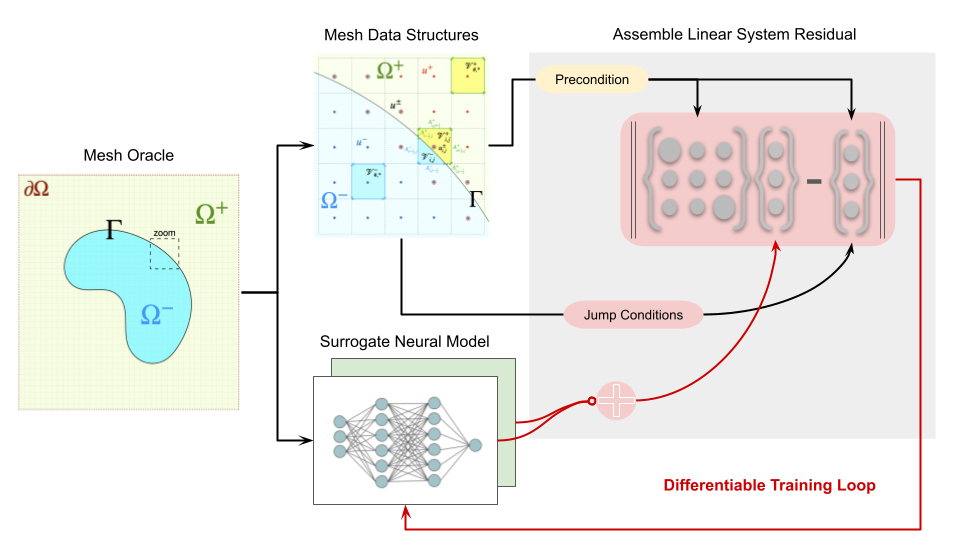
\includegraphics[width=0.85\linewidth]{./figures/jax_dips_paper_v1.png}
	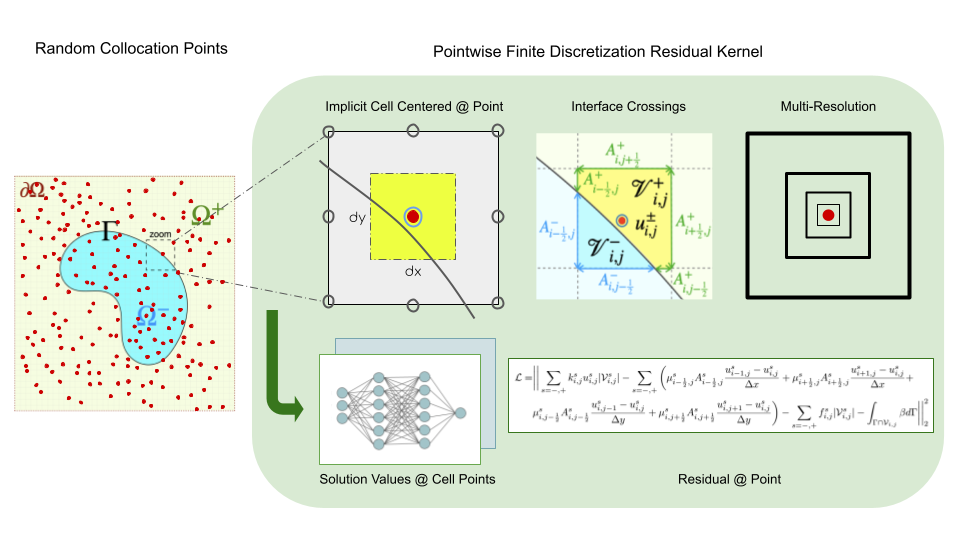
\includegraphics[width=0.85\linewidth]{./figures/jax_dips_paper_kernel.png}
	\caption{Fully classic numerical solver is used to train neural surrogate models. Training occurs in the finite dimensional space spanned by the finite discretization methods.}
	\label{fig:proposal}
\end{figure}
%\begin{figure}[ht]
%	\centering
%	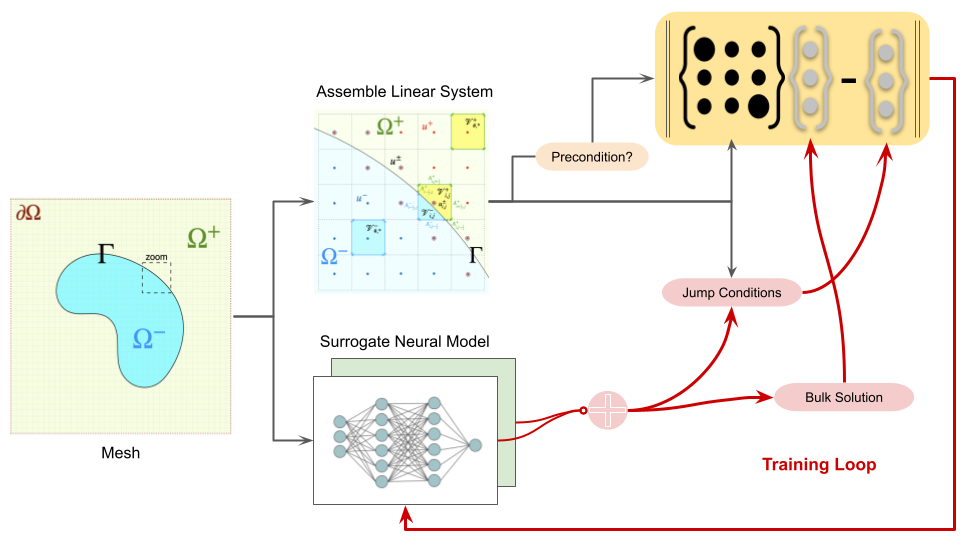
\includegraphics[width=0.85\linewidth]{./figures/jax_dips_paper_v2.png}
%	\caption{Workflow II: stronger merger of the numerical solver with the neural network surrogate model. Training occurs in the finite dimensional space spanned by the finite discretization method.}
%	\label{fig:proposal}
%\end{figure}



\subsection{Neural network approximators for the solution}

In 1987, Hecht and Nielson \cite{hecht1987kolmogorov} applied an improved version of Kolmogorov's 1957 superposition theorem \cite{kolmogorov1957representation}, due to Sprecher \cite{sprecher1965structure}, to the field of neurocomputing and demonstrated that a $3$-layer feedforward neural network (one input layer with $n$ inputs, one hidden layer with $2n+1$ neurons, one output layer) are universal approximators for all \textit{continuous} functions from the $n$-dimensional cube to a finite $m$-dimensional real vector space; \textit{i.e.}, $f: [0,1]^n \rightarrow \mathbb{R}^m $. Recently, Ismailov (2022) \cite{ismailov2022} demonstrated existence of neural networks implementing \textit{discontinuous} functions, however efficient learning algorithms for such networks are not still available. 

The solutions of interfacial PDE problems are discontinuous, with jumps appearing not only in the solution but also in the solution gradient. In light of above considerations, we define two separate neural networks to represent solution in $\Omega^-$ and $\Omega^+$ regions:
\begin{align*}
& u^+ = \mathcal{N}^+(\mathbf{x}): \mathbb{R}^3\cap \Omega^+ \rightarrow \mathbb{R}  & u^- = \mathcal{N}^-(\mathbf{x}): \mathbb{R}^3\cap \Omega^- \rightarrow \mathbb{R}
\end{align*}

We use SIREN neural networks, where we implement fully connected feedforward architecture with \texttt{sin} activation function and the output layer is a single linear neuron. Note that piecewise differentiable nonlinearities such as the \texttt{ReLU} function are inappropriate choices for representing solutions to differential equations. Weights and biases are initialized from a truncated normal distribution with zero mean and unit variance. 




\begin{figure}[ht]
	\centering
	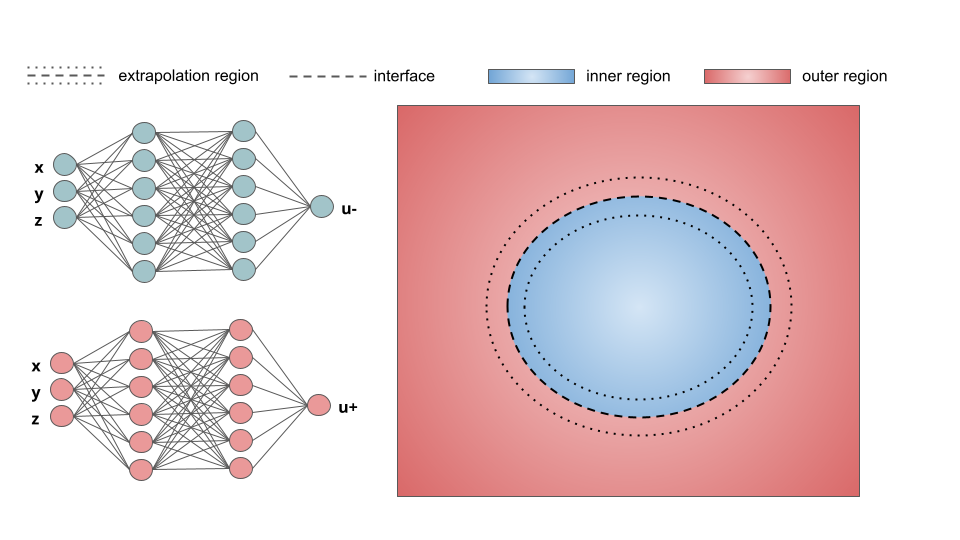
\includegraphics[width=\linewidth]{./figures/neural_network_arch.png}
	\caption{Two neural networks are defined for the two regions of the computational domain.}
	\label{fig:shapes}
\end{figure}

Solution networks are evaluated on grid points while the parameters of these networks are optimized using the loss function. We define the loss function by the mean-squared-error (MSE) of the residual of the discretized partial differential equation with jump conditions derived in section \ref{sec::FD} that is evaluated on the grid points:
\begin{align*}
	&\mathcal{L}(u) = \vert\vert A\hat{u}(\mathbf{x}_{ijk}\in \Omega) - b\vert\vert_2^2 + \textrm{vol}_{\mathcal{C}}\vert\vert \hat{u}(\mathbf{x}_{ijk}\in\partial \Omega) - u(\mathbf{x}_{ijk}\in\partial \Omega)\vert\vert_2^2 
\end{align*}
JAX-DIPS allows for exact computation of the gradient of the loss function using automatic differentiation, \textit{i.e.} $\nabla_u \mathcal{L}(u)$. This is advantageous over existing approximate iterative methods such as GMRES, Conjugate Gradient, \textit{etc}. Therefore, our strategy is to leverage this capability and use more sophisticated optimizers developed in the deep learning community (\textit{e.g.} Adam \cite{kingma2014adam}, RMSProp, \textit{etc}) to minimize the afforementioned loss function with the desired solution vector $\rm u^\ast$ of the PDE problem.










\subsection{Approach I. Finite discretization method fused with regression extrapolation}\label{sec::FD}

For spatial discretizations at the presence of jump conditions we employ the numerical algorithm proposed by \cite{bochkov2020solving} on Cartesian grids. Method of \cite{bochkov2020solving} produces second-order accurate solutions and first-order accuracte gradients in the $L^\infty$-norm, while having a compact stencil that makes it a good candidate for parallelization. Moreover, treatment of the interface jump conditions do not introduce any augmented variables, this preserves the homogeneous structure of the linear system.

Here we use a finite volume discretization equation uniformly for all grid points. At grid points where the finite volumes are crossed by $\rm \Gamma$ we have

\begin{align*}
	 & \sum_{s=-,+}\int_{\Omega^s \cap \mathcal{V}_{i,j}}  k^{s} u^{s} d\Omega -\sum_{s=-,+} \int_{\Omega^s\cap \partial\mathcal{V}_{i,j}} \mu^{s}\partial_{\mathbf{n}^s} u^s  d\Gamma = \sum_{s=-,+}\int_{\Omega^s \cap \mathcal{V}_{i,j}}  f^{s} d\Omega + \int_{\Gamma \cap \mathcal{V}_{i,j}}[\mu\partial_{\mathbf{n}}u]d\Gamma \\
	\intertext{following standard treatment of volumetric integrals and using central differencing for derivatives we obtain in 2D (with trivial 3D extension)}
	 & \sum_{s=-,+} k_{i,j}^s u_{i,j}^{s} |\mathcal{V}_{i,j}^s| - \sum_{s=-,+}\bigg( \mu_{i-\frac{1}{2},j}^s A_{i-\frac{1}{2},j}^s\frac{u_{i-1,j}^s - u_{i,j}^s}{\Delta x}     +   \mu_{i+\frac{1}{2},j}^s A_{i+\frac{1}{2},j}^s\frac{u_{i+1,j}^s - u_{i,j}^s}{\Delta x} +                                                          \\
	 & \mu_{i, j-\frac{1}{2}}^s A_{i, j-\frac{1}{2}}^s\frac{u_{i,j-1}^s - u_{i,j}^s}{\Delta y} + \mu_{i, j+\frac{1}{2}}^s A_{i, j+\frac{1}{2}}^s\frac{u_{i,j+1}^s - u_{i,j}^s}{\Delta y} \bigg)                                                                                                                                     \\
	 & =  \sum_{s=-,+} f_{i,j}^{s} |\mathcal{V}_{i,j}^s| + \int_{\Gamma\cap \mathcal{V}_{i,j}} \beta d\Gamma + \mathcal{O}(\max(\Delta x, \Delta y)^\mathcal{D})
\end{align*}
where $\mathcal{D}$ is the problem dimensionality.

\begin{figure}
	\centering
	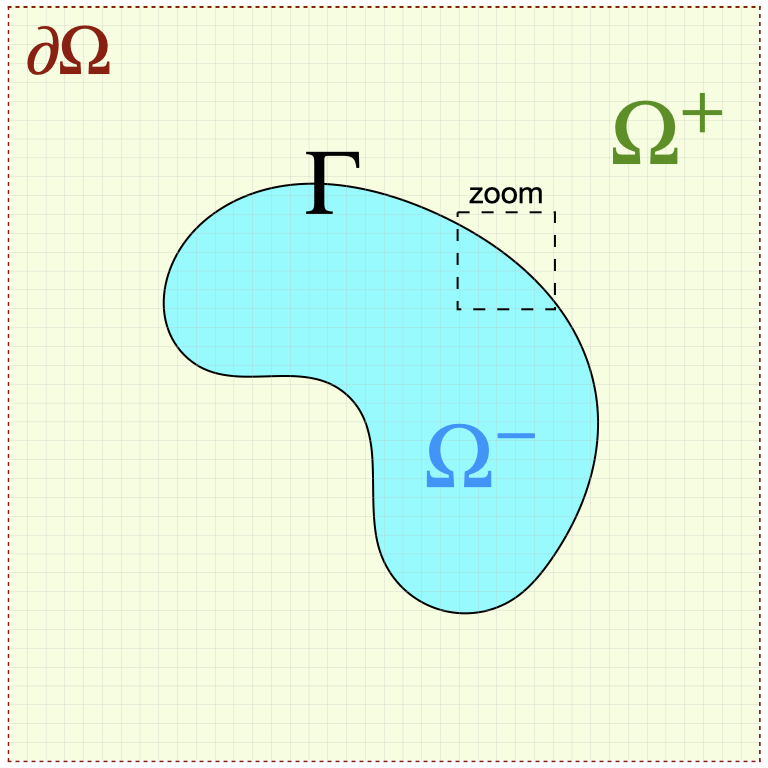
\includegraphics[width=0.45\linewidth]{./figures/grids_full.png}
	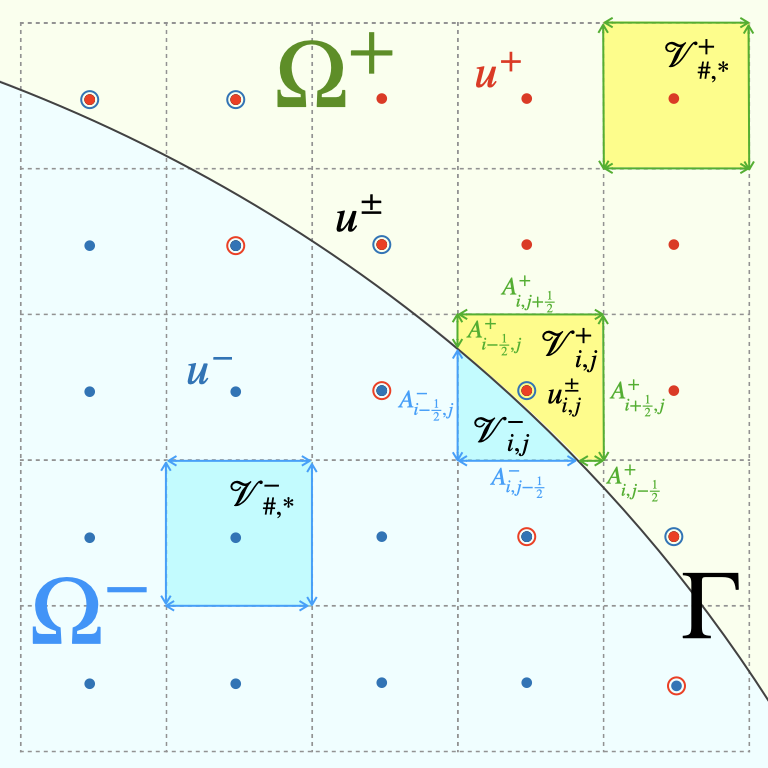
\includegraphics[width=0.45\linewidth]{./figures/grids.png}
	\caption{Notation used in this paper. Close to the interface where finite volumes are crossed by the interface, there are extra degrees of freedom (open circles) that are extrapolations of solutions from each domain to the opposite domain. Jump conditions are implicitly encoded in these extrapolated values.}
	\label{fig:grid}
\end{figure}

Note that far from interface either $s=-$ (for $\mathbf{x}\in \Omega^-$) or $s=+$ (for $\mathbf{x}\in \Omega^+$) is retained. This is automatically considered through zero values for sub-volumes $|\mathcal{V}_{i,j}^+|$ and $|\mathcal{V}_{i,j}^-|$ as well as their face areas. Note that $\mu_{i-1/2,j}^-$ (or $\mu_{i-1/2,j}^+$) corresponds to the value of diffusion coefficient at the middle of segment $A^-_{i-1/2,j}$ (or $A^+_{i-1/2,j}$) respectively, same is true for other edges as well. However, there are extra degrees of freedom on grid points whose finite volumes are crossed by the interface; \textit{i.e.}, see double circles in figure \ref{fig:grid}. \cite{bochkov2020solving} derived analytical expressions for the extra degrees of freedom ($u^+$ in $\Omega^-$ and $u^-$ in $\Omega^+$) in terms of the original degrees of freedom ($u^-$ in $\Omega^-$ and $u^+$ in $\Omega^+$) as well as the jump conditions, this preserves the original $\rm N_x \times N_y$ system size.

In this scheme the basic idea is to extrapolate the jump at grid point from jump condition at the projected point onto the interface using a Taylor expansion: $u^+_{i,j} - u^-_{i,j}=[u]_{\mathbf{r}_{i,j}^{pr}} + \delta_{i,j}(\partial_\mathbf{n}u^+(\mathbf{r}^{pr}_{i,j}) - \partial_\mathbf{n}u^-(\mathbf{r}^{pr}_{i,j})) $. The unknown value ($u^-_{i,j}$ or $u^+_{i,j}$) is obtained based on approximation of the normal derivatives (\textit{i.e.} $\partial_\mathbf{n}u^\pm(\mathbf{r}^{pr}_{i,j})$) which are computed using a least squares calculation on neighboring grid points that are in the fast-diffusion region (referred to as ``Bias Fast'') or in the slow diffusion region (referred to as ``Bias Slow''). This makes two sets of ruls for unknown values $u^\pm_{i,j}$.

In two dimensions and on uniform grids, the gradient operator at the grid cell $(i,j)$ that is crossed by an interface is estimated by a least squares solution given by
\begin{align*}
	 & (\nabla u^\pm)_{i,j} = \mathbf{D}^\pm_{i,j} \begin{bmatrix}
		u_{i-1,j-1} - u^\pm_{i,j} \\
		u_{i,j-1} - u^\pm_{i,j}   \\
		\vdots                    \\
		u_{i+1,j+1} - u^\pm_{i,j}
	\end{bmatrix} & \mathbf{D}^\pm_{i,j} = \big(X^T_{i,j} W^\pm_{i,j} X_{i,j} \big)^{-1} \big( W^\pm_{i,j} X_{i,j} \big)^T
\end{align*}
and
\begin{align*}
	 & W^\pm_{i,j} = \begin{bmatrix}
		 & \omega^\pm_{i,j} (-1,-1) &                         &        &                        \\
		 &                          & \omega^\pm_{i,j} (0,-1) &        &                        \\
		 &                          &                         & \ddots &                        \\
		 &                          &                         &        & \omega^\pm_{i,j} (1,1) \\
	\end{bmatrix} & X_{i,j} = \begin{bmatrix}
		 & -h_x & -h_y \\
		 & 0    & -h_y \\
		 & h_x  & -h_y \\
		 & -h_x & 0    \\
		 & 0    & 0    \\
		 & h_x  & 0    \\
		 & -h_x & h_y  \\
		 & 0    & h_y  \\
		 & h_x  & h_y
	\end{bmatrix}
\end{align*}
and
\begin{equation}
	\omega_{i,j}^\pm (p,q) = \begin{cases}
		1 & (p,q)\in N_{i,j}^\pm \\
		0 & \text{else}
	\end{cases}
\end{equation}
In this case, $D^\pm_{i,j}$ is a $2\times 9$ matrix and we denote each of its $2\times 1$ columns with $d^\pm_{i,j,p,q}$
\begin{align*}
	\mathbf{D}^\pm_{i,j}  = \begin{bmatrix}
		 & d^\pm_{i,j,-1,-1} & d^\pm_{i,j,0,-1} & d^\pm_{i,j,1,-1} & d^\pm_{i,j,-1,0} & d^\pm_{i,j,0,0} & d^\pm_{i,j,1,0} & d^\pm_{i,j,-1,1} & d^\pm_{i,j,0,1} & d^\pm_{i,j,1,1}
	\end{bmatrix}
\end{align*}
The least square coefficients are then obtained by dot product of normal vector with these columns
\begin{align*}
	c^\pm_{i,j,p,q} = \mathbf{n}_{i,j}^T  d^\pm_{i,j,p,q}
\end{align*}
and normal derivative can be computed (noting that $c_{i,j}^\pm =-\sum_{(p,q)\in N_{i,j}^\pm}c_{i,j,p,q}^\pm$)
\begin{align*}
\partial_n u^\pm (\mathbf{r}^{proj}_{i,j})= c_{i,j}^\pm u_{i,j}^\pm + \sum_{(p,q)\in N_{i,j}^\pm} c_{i,j,p,q}^\pm u_{i+p, j+q}^\pm + \mathcal{O}(h) 
\end{align*}

At this point we can define a few intermediate variables at each grid point to simplify the presentation of the method,
\begin{align*}
	 & \zeta_{i,j,p,q}^\pm := \delta_{i,j} \frac{[\mu]}{\mu^\mp}c_{i,j,p,q}^\pm  & \zeta_{i,j}^\pm := -\sum_{(p,q)\in N_{i,j}^\pm} \zeta_{i,j,p,q}^\pm   \\
	 & \gamma_{i,j,p,q}^\pm := \frac{\zeta_{i,j,p,q}^\pm}{1 \pm \zeta^\pm_{i,j}} & \gamma^\pm_{i,j} := -\sum_{(p,q)\in N_{i,j}^\pm} \gamma_{i,j,p,q}^\pm
\end{align*}
where the set of neighboring grid points are
\begin{align*}
	N_{i,j}^\pm = \{(p,q) :\ \ \  p=-1,0,1, \ \ \  q=-1,0,1, \ \ \ (p,q)\neq (0,0), \ \ \ \mathbf{x}_{i+p,j+q}\in \Omega^\pm \}
\end{align*}
and $\delta_{i,j}$ is the signed distance from $\mathbf{x}_{i,j}$ that is computed from the level-set function $\phi(\mathbf{x})$
\begin{align*}
	\delta_{i,j}=\frac{\phi(\mathbf{x}_{i,j})}{|\nabla \phi(\mathbf{x}_{i,j})|}
\end{align*}

\begin{itemize}
	\item Rules based on approximating $\partial_\mathbf{n}u^+(\mathbf{r}^{pr}_{i,j})$:
\end{itemize}
%\begin{equation}
% u_{i,j}^-=\begin{cases}
%    u_{i,j}, & \text{ $\mathbf{x}_{i,j}\in \Omega^-$}\\
%    u_{i,j} - \alpha_1 -\delta_{i,j}\frac{\beta_1}{\mu^{+}} - \delta_{i,j} \frac{[\mu]}{\mu^+} \bigg( \frac{ c_{i,j}^- (u_{i,j} - \alpha_1 - \delta_{i,j}\frac{\beta_1}{\mu^+}) + \sum_{(p,q)\in N_{i,j}^-} c_{i,j,p,q}^- u_{i+p,j+q}  }{ 1 - \delta_{i,j}\frac{[\mu]}{\mu^+}c_{i,j}^- }\bigg), & \text{ $\mathbf{x}_{i,j}\in \Omega^+$}
%  \end{cases}
%\end{equation}
%\begin{equation}
% u_{i,j}^+=\begin{cases}
%    u_{i,j} + \alpha_1 + \delta_{i,j}\frac{\beta_1}{\mu^{+}} - \delta_{i,j} \frac{[\mu]}{\mu^+}\big( c_{i,j}^- u_{i,j}  + \sum_{(p,q)\in N_{i,j}^-} c_{i,j,p,q}^- u_{i+p,j+q} \big), & \text{ $\mathbf{x}_{i,j}\in \Omega^-$}\\
%    u_{i,j}, & \text{ $\mathbf{x}_{i,j}\in \Omega^+$}
%  \end{cases}
%\end{equation}

\begin{equation}
	u_{i,j}^-=\begin{cases}
		u_{i,j}                                                                                                                                                 & \text{ $\mathbf{x}_{i,j}\in \Omega^-$} \\
		u_{i,j} (1 - \gamma_{i,j}^- ) - \sum_{(p,q)\in N_{i,j}^-} \gamma_{i,j,p,q}^- u_{i+p,j+q} - (\alpha + \frac{\delta_{i,j}\beta}{\mu^+})(1-\gamma^-_{i,j}) & \text{ $\mathbf{x}_{i,j}\in \Omega^+$}
	\end{cases}
\end{equation}
\begin{equation}
	u_{i,j}^+=\begin{cases}
		u_{i,j}(1 - \zeta^-_{i,j} ) - \sum_{(p,q)\in N_{i,j}^-} \zeta^-_{i,j,p,q}u_{i+p,j+q}  + \alpha + \delta_{i,j}\frac{\beta}{\mu^+} & \text{ $\mathbf{x}_{i,j}\in \Omega^-$} \\
		u_{i,j}                                                                                                                          & \text{ $\mathbf{x}_{i,j}\in \Omega^+$}
	\end{cases}
\end{equation}
It is useful to cast this in the form of matrix operations through defining intermediate tensors:
\begin{align*}
	 & \boldsymbol{\Gamma}_{i,j} := \begin{bmatrix}
		 & \gamma_{i-1,j+1}^- & \gamma^-_{i,j+1} & \gamma^-_{i+1,j+1} \\
		 & \gamma_{i-1,j}^-   & \gamma^-_{i,j}   & \gamma^-_{i+1,j}   \\
		 & \gamma_{i-1,j-1}^- & \gamma^-_{i,j-1} & \gamma^-_{i+1,j-1}
	\end{bmatrix}, & \boldsymbol{\zeta}_{i,j} := \begin{bmatrix}
		 & \zeta^-_{i-1,j+1} & \zeta^-_{i,j+1} & \zeta^-_{i+1,j+1} \\
		 & \zeta^-_{i-1,j}   & \zeta^-_{i,j}   & \zeta^-_{i+1,j}   \\
		 & \zeta^-_{i-1,j-1} & \zeta^-_{i,j-1} & \zeta^-_{i+1,j-1}
	\end{bmatrix} \\
	 & \mathbf{U}_{i,j} := \begin{bmatrix}
		 & u_{i-1,j+1} & u_{i,j+1} & u_{i+1, j+1} \\
		 & u_{i-1,j}   & u_{i,j}   & u_{i+1, j}   \\
		 & u_{i-1,j-1} & u_{i,j-1} & u_{i+1, j-1}
	\end{bmatrix},          & \mathbf{N}^\pm_{i,j} :=\begin{bmatrix}
		 & \omega_{i,j}^\pm(-1,1)  & \omega_{i,j}^\pm(0,1)  & \omega_{i,j}^\pm(1,1)  \\
		 & \omega_{i,j}^\pm(-1,0)  & 0                      & \omega_{i,j}^\pm(1,0)  \\
		 & \omega_{i,j}^\pm(-1,-1) & \omega_{i,j}^\pm(0,-1) & \omega_{i,j}^\pm(1,-1) \\
	\end{bmatrix}
\end{align*}
where $\mathbf{N^-}$ is a masking filter that passes the values in the negative neighborhood of node $(i,j)$.

We also introduce the Hadamard product $\odot$ between two identical matrices that creates another identical matrix with each entry being elementwise products. Moreover, double contraction of two tensors $A$ and $B$ is defined by $A : B = \sum A \odot B$ which is a scalar value and equals the sum of all entries of the Hadamard product of the tensors; \textit{i.e.}, note $A:A$ is square of Frobenius norm of $A$. Using these notations, the substitution rules read
\begin{equation}
	u_{i,j}^-=\begin{cases}
		u_{i,j}                                                                                                                                                                                                                                                                        & \text{ $\mathbf{x}_{i,j}\in \Omega^-$} \\
		\big(1 + \boldsymbol{\Gamma}^-_{i,j} : \mathbf{N}^-_{i,j}  \big) u_{i,j} -  \big( \boldsymbol{\Gamma}^-_{i,j}  \odot \mathbf{N}^-_{i,j} \big) : \mathbf{U}_{i,j}  - (\alpha + \delta_{i,j}\frac{\beta}{\mu^+}) \big(1 + \boldsymbol{\Gamma}^-_{i,j} : \mathbf{N}^-_{i,j} \big) & \text{ $\mathbf{x}_{i,j}\in \Omega^+$}
	\end{cases}
\end{equation}
\begin{equation}
	u_{i,j}^+=\begin{cases}
		\big(1 + \boldsymbol{\zeta}^-_{i,j} : \mathbf{N}^-_{i,j}   \big) u_{i,j} - \big( \boldsymbol{\zeta}^-_{i,j}  \odot \mathbf{N}^-_{i,j}  \big) : \mathbf{U}_{i,j} + \alpha + \delta_{i,j}\frac{\beta}{\mu^+} & \text{ $\mathbf{x}_{i,j}\in \Omega^-$} \\
		u_{i,j}                                                                                                                                                                                                    & \text{ $\mathbf{x}_{i,j}\in \Omega^+$}
	\end{cases}
\end{equation}



\begin{itemize}
	\item Rules based on approximating $\partial_\mathbf{n}u^-(\mathbf{r}^{pr}_{i,j})$:
\end{itemize}
%\begin{equation}
% u_{i,j}^-=\begin{cases}
%    u_{i,j}, & \text{ $\mathbf{x}_{i,j}\in \Omega^-$}\\
%    u_{i,j} - \alpha_1 -\delta_{i,j}\frac{\beta_1}{\mu^{-}} - \delta_{i,j} \frac{[\mu]}{\mu^-} \big( c_{i,j}^+ u_{i,j} + \sum_{(p,q)\in N_{i,j}^+} c_{i,j,p,q}^+ u_{i+p,j+q} \big) , & \text{ $\mathbf{x}_{i,j}\in \Omega^+$}
%  \end{cases}
%\end{equation}
%\begin{equation}
% u_{i,j}^+=\begin{cases}
%    u_{i,j} + \alpha_1 + \delta_{i,j}\frac{\beta_1}{\mu^{-}} - \delta_{i,j} \frac{[\mu]}{\mu^-} \bigg( \frac{ c_{i,j}^+ (u_{i,j} + \alpha_1 + \delta_{i,j}\frac{\beta_1}{\mu^-}) + \sum_{(p,q)\in N_{i,j}^+} c_{i,j,p,q}^+ u_{i+p,j+q}  }{ 1 + \delta_{i,j}\frac{[\mu]}{\mu^-}c_{i,j}^+ }\bigg), & \text{ $\mathbf{x}_{i,j}\in \Omega^-$} \\
%    u_{i,j}, & \text{ $\mathbf{x}_{i,j}\in \Omega^+$}\\
%  \end{cases}
%\end{equation}
\begin{equation}
	u_{i,j}^-=\begin{cases}
		u_{i,j}                                                                                                                        & \text{ $\mathbf{x}_{i,j}\in \Omega^-$} \\
		u_{i,j} (1-\zeta^+_{i,j}) - \sum_{(p,q)\in N_{i,j}^+} \zeta_{i,j,p,q}^+ u_{i+p,j+q} - \alpha - \delta_{i,j}\frac{\beta}{\mu^-} & \text{ $\mathbf{x}_{i,j}\in \Omega^+$}
	\end{cases}
\end{equation}
\begin{equation}
	u_{i,j}^+=\begin{cases}
		u_{i,j}(1 - \gamma^+_{i,j}) - \sum_{(p,q)\in N^+_{i,j}} \gamma^+_{i,j,p,q} u_{i+p, j+q} + (\alpha + \delta_{i,j}\frac{\beta}{\mu^-})(1 - \gamma^+_{i,j}) & \text{ $\mathbf{x}_{i,j}\in \Omega^-$} \\
		u_{i,j}                                                                                                                                                  & \text{ $\mathbf{x}_{i,j}\in \Omega^+$} \\
	\end{cases}
\end{equation}
in matrix notation we have
\begin{equation}
	u_{i,j}^-=\begin{cases}
		u_{i,j}                                                                                                                                                                                                 & \text{ $\mathbf{x}_{i,j}\in \Omega^-$} \\
		\big(1 + \boldsymbol{\zeta}^+_{i,j} : \mathbf{N}^+_{i,j}\big) u_{i,j}  -  \big( \boldsymbol{\zeta}^+_{i,j} \odot \mathbf{N}^+_{i,j} \big) : \mathbf{U}_{i,j} - \alpha - \delta_{i,j}\frac{\beta}{\mu^-} & \text{ $\mathbf{x}_{i,j}\in \Omega^+$}
	\end{cases}
\end{equation}
\begin{equation}
	u_{i,j}^+=\begin{cases}
		\big(1 + \boldsymbol{\Gamma}^+_{i,j} : \mathbf{N}^+_{i,j}\big) u_{i,j} - \big( \boldsymbol{ \Gamma}^+_{i,j} \odot  \mathbf{N}^+_{i,j}  \big) : \mathbf{U}_{i,j} + (\alpha + \delta_{i,j}\frac{\beta}{\mu^-})\big(1 + \boldsymbol{\Gamma}^+_{i,j} : \mathbf{N}^+_{i,j} \big) & \text{ $\mathbf{x}_{i,j}\in \Omega^-$} \\
		u_{i,j}                                                                                                                                                                                                                                                                     & \text{ $\mathbf{x}_{i,j}\in \Omega^+$} \\
	\end{cases}
\end{equation}



\begin{algorithm}
	\caption{Bias Slow approximation of the non-existing solution value on a grid point based on existing solution values in its neighborhood. The notation is used for $u_{i,j}^\pm=B_{i,j}^\pm : \mathbf{U}_{i,j}+r_{i,j}^\pm$.}\label{euclid}
	\begin{algorithmic}[1]
		\Procedure{Bias Slow}{}
		\If {$\Gamma \cap \mathcal{C}_{i,j}= \emptyset$}
		\State $B_{i,j}^\pm=\begin{bmatrix}
				0 & 0 & 0 \\
				0 & 1 & 0 \\
				0 & 0 & 0 \\
			\end{bmatrix};\ \ r^\pm_{i,j}=0$
		\Else
		\If {$\mu_{i,j}^- > \mu_{i,j}^+$}
		\If {$\phi_{i,j}\ge 0$}
		\State $B_{i,j}^+=\begin{bmatrix}
				0 & 0 & 0 \\
				0 & 1 & 0 \\
				0 & 0 & 0 \\
			\end{bmatrix};\ \ r^+_{i,j}=0$
		\State $B_{i,j}^-=\begin{bmatrix}
				-\gamma_{i,j,-1,1}^-  & -\gamma_{i,j,0,1}^-  & -\gamma_{i,j,1,1}^-  \\
				-\gamma_{i,j,-1,0}^-  & 1-\gamma^-_{i,j}     & -\gamma_{i,j,1,0}^-  \\
				-\gamma_{i,j,-1,-1}^- & -\gamma_{i,j,0,-1}^- & -\gamma_{i,j,1,-1}^- \\
			\end{bmatrix};\ \ r^-_{i,j}=-(\alpha_{i,j}^{proj} + \delta_{i,j}\frac{ \beta_{i,j}^{proj}}{\mu_{proj}^+}) (1 - \gamma_{i,j}^-)$
		\Else

		\State $B_{i,j}^+=\begin{bmatrix}
				-\zeta_{i,j,-1,1}^-  & -\zeta_{i,j,0,1}^-  & -\zeta_{i,j,1,1}^-  \\
				-\zeta_{i,j,-1,0}^-  & 1-\zeta^-_{i,j}     & -\zeta_{i,j,1,0}^-  \\
				-\zeta_{i,j,-1,-1}^- & -\zeta_{i,j,0,-1}^- & -\zeta_{i,j,1,-1}^- \\
			\end{bmatrix};\ \ r^+_{i,j}=\alpha_{i,j}^{proj} + \delta_{i,j}\frac{ \beta_{i,j}^{proj}}{\mu_{proj}^+}$

		\State $B_{i,j}^-=\begin{bmatrix}
				0 & 0 & 0 \\
				0 & 1 & 0 \\
				0 & 0 & 0 \\
			\end{bmatrix};\ \ r^-_{i,j}=0$

		\EndIf

		\Else




		\If {$\phi_{i,j}\ge 0$}
		\State $B_{i,j}^+=\begin{bmatrix}
				0 & 0 & 0 \\
				0 & 1 & 0 \\
				0 & 0 & 0 \\
			\end{bmatrix};\ \ r^+_{i,j}=0$
		\State $B_{i,j}^-=\begin{bmatrix}
				-\zeta_{i,j,-1,1}^+  & -\zeta_{i,j,0,1}^+  & -\zeta_{i,j,1,1}^+  \\
				-\zeta_{i,j,-1,0}^+  & 1-\zeta^+_{i,j}     & -\zeta_{i,j,1,0}^+  \\
				-\zeta_{i,j,-1,-1}^+ & -\zeta_{i,j,0,-1}^+ & -\zeta_{i,j,1,-1}^+ \\
			\end{bmatrix};\ \ r^-_{i,j}=\alpha_{i,j}^{proj} + \delta_{i,j}\frac{ \beta_{i,j}^{proj}}{\mu_{proj}^-}$
		\Else

		\State  $B_{i,j}^+=\begin{bmatrix}
				-\gamma_{i,j,-1,1}^+  & -\gamma_{i,j,0,1}^+  & -\gamma_{i,j,1,1}^+  \\
				-\gamma_{i,j,-1,0}^+  & 1-\gamma^+_{i,j}     & -\gamma_{i,j,1,0}^+  \\
				-\gamma_{i,j,-1,-1}^+ & -\gamma_{i,j,0,-1}^+ & -\gamma_{i,j,1,-1}^+ \\
			\end{bmatrix};\ \ r^+_{i,j}=(\alpha_{i,j}^{proj} + \delta_{i,j}\frac{ \beta_{i,j}^{proj}}{\mu_{proj}^-}) (1 - \gamma_{i,j}^+)$

		\State $B_{i,j}^-=\begin{bmatrix}
				0 & 0 & 0 \\
				0 & 1 & 0 \\
				0 & 0 & 0 \\
			\end{bmatrix};\ \ r^-_{i,j}=0$

		\EndIf


		\EndIf

		\EndIf

		%\BState \emph{top}:
		%\If {$i > \textit{stringlen}$} \Return false
		%\EndIf
		%\State $j \gets \textit{patlen}$
		%\BState \emph{loop}:
		%\If {$\textit{string}(i) = \textit{path}(j)$}
		%\State $j \gets j-1$.
		%\State $i \gets i-1$.
		%\State \textbf{goto} \emph{loop}.
		%\State \textbf{close};
		%\EndIf
		%\State $i \gets i+\max(\textit{delta}_1(\textit{string}(i)),\textit{delta}_2(j))$.
		%\State \textbf{goto} \emph{top}.
		\EndProcedure
	\end{algorithmic}
\end{algorithm}


\subsection{Approach II. Finite discretization method fused with neural extrapolation}
Our proposed hybrid PDE solver is based on the observation that the neural network models for negative and positive domains can be explicitly used as interpolation and extrapolation functions within the finite discretization schemes.  

The basic idea of the finite discretization method of section \ref{sec::FD} is to impose the jump conditions on the already-available grid points in the computational cells that are crossed by the interface, instead of aspiring to impose the jump conditions exactly on the interface itself. This is achieved by a Taylor expansion to project the interfacial jump conditions onto adjacent grid points. Using the neural network models for solutions, we are able to naturally evaluate extensions of the solution functions in a banded region around the interface as illustrated in figure \ref{fig:shapes}.


Starting from the jump conditions, for points on the interface, $\mathbf{x}\in \Gamma$, we have
\begin{align*}
u^+ - u^- &= \alpha\\
\mu^+\partial_n u^+ - \mu^- \partial_n u^- &= \beta
\end{align*}
and after Taylor expansion in the normal direction we obtain on the adjacent grid points $(i,j)$
\begin{align}
u^+_{i,j} - u^-_{i,j}=[u]_{\mathbf{r}_{i,j}^{pr}} + \delta_{i,j}(\partial_\mathbf{n}u^+(\mathbf{r}^{pr}_{i,j}) - \partial_\mathbf{n}u^-(\mathbf{r}^{pr}_{i,j})) \label{eq::taylorexpandjump}
\end{align}
which explicitly incorporates the jump condition in the solutions. To incorporate the jump condition in fluxes we can rewrite either of the normal gradients in terms of the other 
\begin{align*}
\partial_\mathbf{n}u^+(\mathbf{r}^{pr}_{i,j}) &= \frac{\mu^-}{\mu^+}\partial_\mathbf{n}u^-(\mathbf{r}^{pr}_{i,j}) + \frac{\beta}{\mu^+}\\
\partial_\mathbf{n}u^-(\mathbf{r}^{pr}_{i,j}) &= \frac{\mu^+}{\mu^-}\partial_\mathbf{n}u^+(\mathbf{r}^{pr}_{i,j}) - \frac{\beta}{\mu^-} 
\end{align*}
which leads to two relationships among predictions of the two neural networks at each grid point in the banded extrapolation region
\begin{align}
u^+_{i,j} - u^-_{i,j}=\alpha(\mathbf{r}_{i,j}^{pr}) + \delta_{i,j}\bigg(\big(\frac{\mu^-}{\mu^+}-1\big)\partial_\mathbf{n}u^-(\mathbf{r}^{pr}_{i,j}) + \frac{\beta(\mathbf{r}_{i,j}^{pr})}{\mu^+} \bigg)  \label{eq::extrapolate1}\\
u^+_{i,j} - u^-_{i,j}=\alpha(\mathbf{r}_{i,j}^{pr}) + \delta_{i,j}\bigg(\big(1-\frac{\mu^+}{\mu^-}\big)\partial_\mathbf{n}u^+(\mathbf{r}^{pr}_{i,j}) + \frac{\beta(\mathbf{r}_{i,j}^{pr})}{\mu^-} \bigg) \label{eq::extrapolate2}
\end{align}

Note that we are representing solution functions, $\hat{u}^\pm(\mathbf{r})$, with neural networks where computing the normal derivatives is trivial using automatic differentiation of the network along the normal directions. In contrast to finite discretization methods, solutions at off-grid points is readily accessible by simply evaluating the neural network function at any desired points. Note that we can compute the projected location on the interface starting from each grid point $(i,j)$ using the level-set function:
\begin{align*}
\mathbf{r}_{ij}^{proj}=\mathbf{r}_{ij} - \delta_{i,j} \mathbf{n}_{i,j}
\end{align*}


In the second approach, the loss function remains as before, except the unknown $u^\pm$ values are derived using equations \ref{eq::extrapolate1}--\ref{eq::extrapolate2}, instead of computing a regression-based extrapolation function based on the points in the neighborhood of interface cells: 

\begin{align*}
\mathcal{L} = & \bigg\vert\bigg\vert \sum_{s=-,+} k_{i,j}^s u_{i,j}^{s} |\mathcal{V}_{i,j}^s| - \sum_{s=-,+}\bigg( \mu_{i-\frac{1}{2},j}^s A_{i-\frac{1}{2},j}^s\frac{u_{i-1,j}^s - u_{i,j}^s}{\Delta x}     +   \mu_{i+\frac{1}{2},j}^s A_{i+\frac{1}{2},j}^s\frac{u_{i+1,j}^s - u_{i,j}^s}{\Delta x} +                                                          \\
	 & \mu_{i, j-\frac{1}{2}}^s A_{i, j-\frac{1}{2}}^s\frac{u_{i,j-1}^s - u_{i,j}^s}{\Delta y} + \mu_{i, j+\frac{1}{2}}^s A_{i, j+\frac{1}{2}}^s\frac{u_{i,j+1}^s - u_{i,j}^s}{\Delta y} \bigg)  -  \sum_{s=-,+} f_{i,j}^{s} |\mathcal{V}_{i,j}^s| - \int_{\Gamma\cap \mathcal{V}_{i,j}} \beta d\Gamma \bigg\vert\bigg\vert_2^2
\end{align*}


There is a major downside with this approach, that we need to compute second-order derivatives of the network during training. This slows down convergence dramatically, and the time-to-solution increases with increasing the number of neural layers. As a result we use 2 hidden layers for this approach with 10 neurons in each layer.




\subsection{Approach III. Penalty minimization method}
Physics-informed neural networks (PINNs) are based on minimizing a penalty function on evaluated on a point cloud, where the actual PDE constitutes the residual and automatic differentiation is used to compute the spatial derivaties in the PDE. Each of the two relations \ref{eq::extrapolate1}--\ref{eq::extrapolate2} offers an extra residual term that can be used to penalize the loss function in PINNs
\begin{align}
\mathcal{L}_{interface} &= \bigg|\bigg| u^+_{i,j} - u^-_{i,j} - \alpha(\mathbf{r}_{i,j}^{pr}) - \delta_{i,j}\bigg(\big(\frac{\mu^-}{\mu^+}-1\big)\partial_\mathbf{n}u^-(\mathbf{r}^{pr}_{i,j}) + \frac{\beta(\mathbf{r}_{i,j}^{pr})}{\mu^+} \bigg) \bigg|\bigg|_2^2 \\
\intertext{or}
\mathcal{L}_{interface} &= \bigg|\bigg| u^+_{i,j} - u^-_{i,j} - \alpha(\mathbf{r}_{i,j}^{pr}) - \delta_{i,j}\bigg(\big(1-\frac{\mu^+}{\mu^-}\big)\partial_\mathbf{n}u^+(\mathbf{r}^{pr}_{i,j}) + \frac{\beta(\mathbf{r}_{i,j}^{pr})}{\mu^-} \bigg) \bigg|\bigg|_2^2
 \label{eq::interfaceLoss}
\end{align}


Far from interface, the usual procedure for physics-informed neural networks is applicable, namely,
\begin{align*}
\mathcal{L}_{bulk} &= \bigg|\bigg| k^{\pm}u^{\pm} - \nabla \cdot (\mu^{\pm}\nabla u^\pm) - f^{\pm} \bigg|\bigg|_2^2 \\
\mathcal{L}_{boundary} &= \bigg|\bigg|u(\mathbf{r}_{bc}) - \hat{u}(\mathbf{r}_{bc})\bigg|\bigg|_2^2
\end{align*}
hence, the overall loss function for this class of problems shall be
\begin{align*}
\mathcal{L} = \mathcal{L}_{bulk} + \mathcal{L}_{boundary} + \mathcal{L}_{interface}
\end{align*}



\section{Optimization scheme}


\subsection{Preconditioners are ideal network regularizers}
Finite discretization methods lead to solving a linear algebraic system with gaurantees on convergence and accuracies. The geometric irregularities and fine-grain details of the system often lead to bad condition number for the linear system, which can be remedied by advanced preconditioners. Preconditioners are a powerful technique to accelerate convergence of tradional numerical linear algebraic solvers. Given a poorly conditioned linear system $Ax=b$ one can obtain an equivalent system $\hat{A}\hat{x}=\hat{b}$ with accelerated convergence rate when using iterative gradient based methods. For the conjugate gradient method convergence iteration is proportional to $\sqrt{\kappa(A)}$ where $\kappa(A)$ is the condition number of matrix $A$. This is achieved by mapping the linear system with a nonsingular matrix $M$ into a new space $M^{-1} A x = M^{-1}b$ where $M^{-1}A$ has more regular spread of eigenvalues, hence a better condition number. The precondition matrix $M$ should approximate $A^{-1}$ such that $\vert I - M^{-1}A\vert < 1$. The simplest choice is the Jacobi prconditioner which amounts to using the diagonal part of $A$ as the preconditioner, $M=diag(A)$.



Intuitively, condition number is caused by a separation of scales for geometric lengthscales or material properties that underly the solution patterns. One of the strengths of the presented approach is to readily enable usage of preconditioners for training neural network surrogate models. The workflow for training neural network surrogate models for PDEs with discontinuities is illustrated in figure \ref{fig:proposal}.

In this work we use the Jacobi pre-conditioner. Basically, every element of the left-hand-side ($A u$) and right-hand-side ($b$) vectors are divided by the coefficient of the diagonal term of the matrix given by:
\begin{align*}
a_{ii} = \sum_{s=-,+} \bigg( k_{i,i}^s \vert \mathcal{V}_{i,i}^s\vert + (\mu_{i-\frac{1}{2},i}^s A_{i-\frac{1}{2},i}^s +  \mu_{i+\frac{1}{2},i}^s A_{i+\frac{1}{2},i}^s ) / \Delta x 
+  (\mu_{i, i-\frac{1}{2}}^s A_{i, i-\frac{1}{2}}^s +  \mu_{i, i+\frac{1}{2}}^s A_{i, i+\frac{1}{2}}^s ) / \Delta y \bigg)
\end{align*}
Note that we never explicitly compute the matrix, instead we compute the effect of matrix product of $A u$.  






\subsection{Learning rate scheduling}
First order methods are slow but cheap; second order methods are fast but expensive. In \texttt{JAX-DIPS} we primarily utilize first order optimization methods such as Adam, RMSProp, etc. Second order methods such as Newton or BFGS are certainly faster convergence but require much more memory. Traditionally used GMRES or Conjugate Gradient methods for sparse linear systems are somewhere between first order and second order optimization methods that are based on build a basis vectors by computing gradients that are conjugate to each other $\mathbf{p}_j^T A \mathbf{p}_i=0$ and will converge to the solution in at most $n$ steps; \textit{i.e.}, at most the solution vector is spanned in the full basis.


%\subsubsection{Gradient based optimization with learning rate annealing}

We found that starting from a zero guess for the solution it is important to start from a large learning rate and gradually decay the learning rate in a process of exponential annealing. For this purpose, we use the exponential decay scheduler provided by \texttt{Optax} \cite{optax2020github} to control the learning rate in the Adam \cite{kingma2014adam} optimizer:
\begin{align*}
r_{k} = r_0 \alpha^{k / T}
\end{align*}
where $r_k$ is the learning rate at step $k$ of optimization, $\alpha<1$ is the decay rate, and $T$ is the decay count-scale. By default, we set $T=100$, $\alpha=0.975$, starting from an initial value of $r_0=10^{-2}$ and clip gradients by maximum global gradient norm (to a value $1$) \cite{gradClipping} before applying the Adam updates in each step. We note a larger decay rate, \textit{e.g.} $\alpha=0.98$, leads to small oscillations after $10000$ steps and although similar levels of accuracy can be achieved at much less iterations, here we report results with the more robust decay rate. %See figure \ref{fig::optimization} for an example of loss evolution during optimization.

%\begin{figure}[ht]
%\centering
%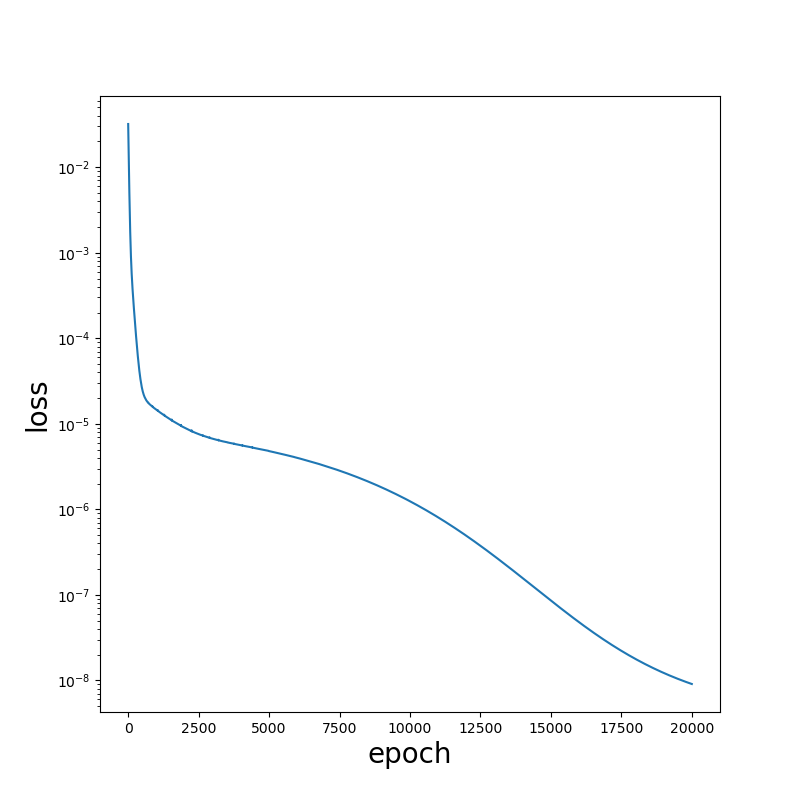
\includegraphics[width=0.85\linewidth]{figures/poisson_solver_loss_with_annealing.png}
%\caption{Effect of annealing to dampen learning rate with number of epochs. }
%\label{fig::optimization}
%\end{figure}




\subsection{Domain switching optimization scheme}
The linear system suffers from worse condition number in the domain with more variability in diffusion coefficient, or where diffusion coefficient is larger; \textit{i.e.,} the fast region. This leads to regionally unbalanced solution error where the overall error is systematically lopsided by the faster diffusion region. 

We found this problem can be drastically improved by interleaving region-specific optimization epochs in the training pipeline, where only one of the networks is updated based on the loss computed in the its region. See algorithm \ref{switching} for details of the algorithm.

\begin{algorithm}
	\caption{Domain switching method. Switching interval is $\tau$.}\label{switching}
	\begin{algorithmic}[1]
		\Procedure{Domain Switching Optimization}{}
		
		\For {$epoch$ in $0\cdots$ N}	
			\State $region = Region (epoch)$
			
			\If {$region > 0$}
				\If {$\mu^- > \mu^+$}
					\State optimize $u^-_{NN}$ in $\Omega^-$ given fixed $u^+_{NN}$  
				\Else
					\State optimize $u^+_{NN}$ in $\Omega^+$ given fixed $u^-_{NN}$ 
				\EndIf	
			\EndIf	
			\\
			\If {$region==0$}
				\State optimize both networks in $\Omega^- \cup \Omega^+$ 
			\EndIf	
			\\
			\If {$region < 0$}
				\If {$\mu^- < \mu^+$}
					\State optimize $u^-_{NN}$ in $\Omega^-$ given fixed $u^+_{NN}$  
				\Else
					\State optimize $u^+_{NN}$ in $\Omega^+$ given fixed $u^-_{NN}$ 
				\EndIf					
			\EndIf	
				
			
		\EndFor

		\EndProcedure
		\\
		\Procedure{Region}{epoch}
			\If {$mode == \textrm{whole region} \rightarrow \textrm{fast region}$}
				\State $region = epoch\ \%\ \tau $ 
			\EndIf
			\If {$mode == \textrm{fast region}\rightarrow \textrm{whole region} \rightarrow \textrm{slow region}$}
				\State $region = \tau // 2 - epoch\ \%\ \tau  $ 
			\EndIf
		\EndProcedure
	\end{algorithmic}
\end{algorithm}




\section{Numerical Examples}

We consider solution to the problem
\begin{align*}
	 & k^{\pm}u^{\pm} - \nabla \cdot (\mu^{\pm}\nabla u^\pm)=f^{\pm}, & \mathbf{x}\in\Omega^\pm \\
	 & [u]=\alpha,                                                    & \mathbf{x} \in \Gamma   \\
	 & [\mu \partial_{\mathbf{n}}u]=\beta,                            & \mathbf{x} \in \Gamma
\end{align*}


In both cases a pair of neural networks with architecture $3\times 20 \times 20 \times 20 \times 20  \times 20 \times 1$ are used with \texttt{tanh} activation functions for hidden layers and linear output neuron. There are $3,562$ trainable parameters (\textit{i.e.}, weights and biases) in the model.

%
%\subsection{No interface, $\Gamma=\emptyset $}
%We set the level-set function to $\phi(\mathbf{x})=\sqrt{x^2 + y^2 + z^2} + 0.5$ within a domain $\Omega:[-1,1]^3$ characterizing absence of all jump conditions. Using the method of manufactured solutions, we construct the following Poisson problem for an exact solution $u(\mathbf{x}) = \sin(y)\cos(x)$ with appropriate Dirichlet boundary conditions:
%\begin{align*}
%	 - \Delta u &=2\sin(y)\cos(x), & \mathbf{x}\in\Omega\\
%	 u(\mathbf{x}) &= \sin(y)\cos(x), &\mathbf{x}\in \partial \Omega
%\end{align*}
%with \texttt{Adam} optimizer starting from an initial condition $\hat{u}(\mathbf{x};t=0)=y$ which does not satisfy the system of equations.



%\subsection{Interface, $\Gamma\neq \emptyset$}
\subsection{Case I.}
%We consider the example 4.6 of the Voronoi-Interface Method (VIM) of Guittet et al 2015 \cite{guittet2015solving} where a sphere $\phi(\mathbf{x})=\sqrt{x^2 + y^2 + z^2} - 0.5$ is centered in a box $\Omega:[-1,1]^3$ with the exact solution
We consider a sphere $\phi(\mathbf{x})=\sqrt{x^2 + y^2 + z^2} - 0.5$ centered in a box $\Omega:[-1,1]^3$ with the exact solution
\begin{align*}
& u^-(x,y,z)=e^{z}, & \phi(\mathbf{x})<0\\
& u^+(x,y,z)=\cos(x)\sin(y), & \phi(\mathbf{x})\ge 0
\end{align*}
and the diffusion coefficient
\begin{align*}
\mu^-(x,y,z)&=y^2 \ln(x+2) + 4 &\phi(\mathbf{x})<0 \\
\mu^+(x,y,z)&=e^{-z} &\phi(\mathbf{x})\ge 0 
\end{align*}
that imply
\begin{align*}
&f^-(x,y,z)=-[y^2\ln(x+2) + 4] e^{z} &\phi(\mathbf{x})< 0\\
&f^+(x,y,z)=2\cos(x)\sin(y)e^{-z} &\phi(\mathbf{x})\ge 0
\end{align*}

Table 8 of \cite{guittet2015solving} reports convergence results for the solution and its gradient over the surface of the sphere in the $L^\infty$-norm, here we report similar results for comparison with VIM. Order of convergence, denoted by $p$, is computed by doubling the number of grid points in every dimension and measuring the $L^\infty$ error of solution and its gradient over all the grid points in the domain:
\begin{align*}
&\frac{\textrm{err}(2h)}{\textrm{err}(h)}=2^p \rightarrow p = \log_2\bigg(\frac{\textrm{err}(2h)}{\textrm{err}(h)}\bigg)  & h=\min(h_x,h_y,h_z)
\end{align*}


%\begin{table}[ht]
%\begin{center}
%\begin{tabular}{|l||ll|ll|ll|ll|c|}
%\hline
%& \multicolumn{2}{c|}{VIM}& \multicolumn{2}{c|}{JAX-DIPS} & \multicolumn{2}{|c|}{VIM}& \multicolumn{3}{c|}{JAX-DIPS}\\
%\hline
%$\rm N_{x,y,z}$   &   Solution    &   Order   &   Solution   &   Order &   Gradient    &   Order   &   Gradient   &   Order & t (sec/epoch) \\
%\hline
%$2^3$ & $3.61\times 10^{-3}$ & -         & $9.49\times 10^{-1}$ & -      & $1.13\times 10^{-2}$ & -      & $2.38$               & -      & 180\\ 
%$2^4$ & $1.21\times 10^{-3}$ & $1.58$    & $1.56\times 10^{-1}$ & $2.60$ & $7.69\times 10^{-3}$ & $0.56$ & $4.80\times 10^{-1}$ & $2.31$ & 274\\ 
%$2^5$ & $3.04\times 10^{-4}$ & $1.99$    & - & - & $3.83\times 10^{-3}$ & $1.01$ & - & - &  \\ 
%$2^6$ & $7.74\times 10^{-5}$ & $1.98$    & $8.86\times 10^{-2}$ & - & $2.43\times 10^{-3}$ & $0.66$ & $5.73\times 10^{-1}$ & -& 1.45\\ 
%$2^7$ & $1.97\times 10^{-5}$ & $1.98$    & - & - & $1.24\times 10^{-3}$ & $0.98$ & - & -&\\ \hline
%\end{tabular}
%\caption{Convergence on the solution and its gradient. VIM values are the $L^\infty$-norm over the surface of the sphere. We report $L^\infty$-norm of solution and its gradient evaluated everywhere in the domain (more conservative). Rightmost column reports the overall time to solution for \texttt{JAX-DIPS} which constitutes $10,000$ epochs in each case.}
%\end{center}
%\end{table}
\begin{table}[ht]
\begin{center}
\begin{tabular}{|l||ll|ll|c|c|}
\hline
regress $\partial_n$ & \multicolumn{2}{c|}{RMSE}& \multicolumn{2}{c|}{$L^\infty$} & \multicolumn{2}{c|}{GPU Statistics} \\
\hline
$\rm N_{x,y,z}$   &   Solution    &   Order   &   Solution   &   Order & t (sec/epoch) & VRAM (GB)\\
\hline 
$2^3$ & $3.7\times 10^{-2}$ &  -        & $3.25\times 10^{-1}$  &   -     & $0.0306$ & $1.05$ \\
$2^4$ & $7.1\times 10^{-3}$ &  $2.38$   & $1.1\times 10^{-1}$   & $1.56$  & $0.056$  & $1.72$ \\ 
$2^5$ & $5.9\times 10^{-3}$ &  $0.27$   & $8.36 \times 10^{-2}$ & $0.4$   & $0.053$  & $2.15$ \\ 
$2^6$ & $4.1\times 10^{-3}$ &  $0.53$   & $6.44\times 10^{-2}$  & $0.38$  & $0.287$  & $5.57$ \\ 
$2^7$ & $2.64\times 10^{-3}$&  $0.64$   & $3.53\times 10^{-2}$  & $0.87$  & $2.125$ & $32.1$ \\ \hline
\end{tabular}
\begin{tabular}{|l||ll|ll|c|c|}
\hline
neural $\partial_n$ & \multicolumn{2}{c|}{RMSE}& \multicolumn{2}{c|}{$L^\infty$} & \multicolumn{2}{c|}{GPU Statistics} \\
\hline
$\rm N_{x,y,z}$   &   Solution    &   Order   &   Solution   &   Order & t (sec/epoch) & VRAM (GB)\\
\hline 
$2^3$ & $ $ &  -     & $ $  &   -   & $ $ & $ $ \\
$2^4$ & $ $ &  $ $   & $ $  & $ $   & $ $ & $ $ \\ 
$2^5$ & $ $ &  $ $   & $ $  & $ $   & $ $ & $ $ \\ 
$2^6$ & $ $ &  $ $   & $ $  & $ $   & $ $ & $ $ \\ 
$2^7$ & $ $ &  $ $   & $ $  & $ $   & $ $ & $ $ \\ \hline
\end{tabular}
\caption{Convergence on the solution using the regression-based solver. We report $L^\infty$-norm error as well as root-mean-squared-error (RMSE) of the solution field evaluated everywhere in the domain. Rightmost column reports the overall time to solution for \texttt{JAX-DIPS} which constitutes $10,000$ epochs in each case and the initial compilation time of jaxpressions. The neural network has $982$ trainable parameters. In each case GPU compute occupancy is at $100\%$ on a single NVIDIA RTX A6000 GPU. The neural method has 2 hidden layers with 10 neurons each, overall 322 trainable parameteres. The regression-based method has 5 hidden layers with 10 neurons each, overall 928 trainable parameters.}
\end{center}
\end{table}




After $\rm 10,000$ epochs on a grid of $16\times 16 \times 16$ the $\rm L^\infty$-norm error of the solution is $1.1\times 10^{-1}$, corresponding to a $10\%$ relative error in the solution.


\begin{figure}
	\centering
	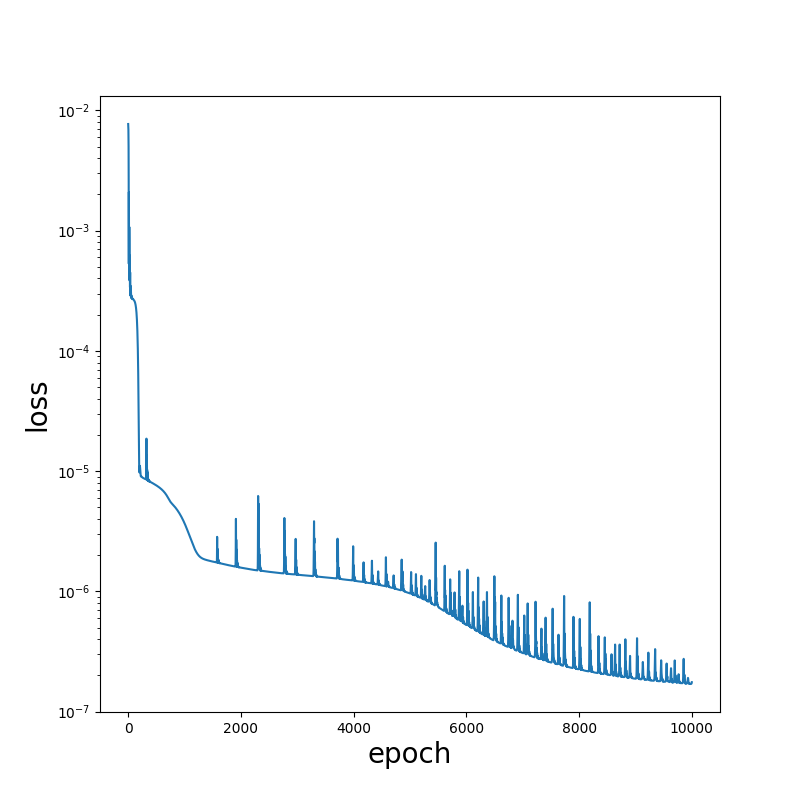
\includegraphics[width=0.49\linewidth]{./figures/poisson_solver_loss_sphere_128x128x128.png}
	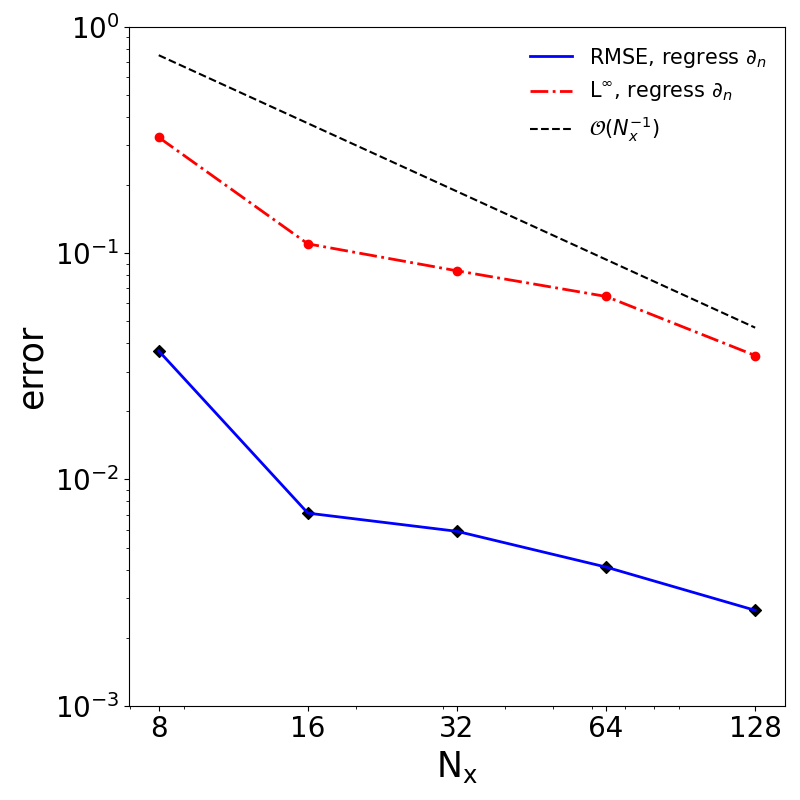
\includegraphics[width=0.45\linewidth]{./figures/case_I_regression.png}
	\caption{Loss evolution with epochs for the sphere of $16\times 16\times 16$ grid (left) and different accuracy measures at 5 resolutions (right).}
	\label{fig:losses}
\end{figure}


\begin{figure}
	\centering
	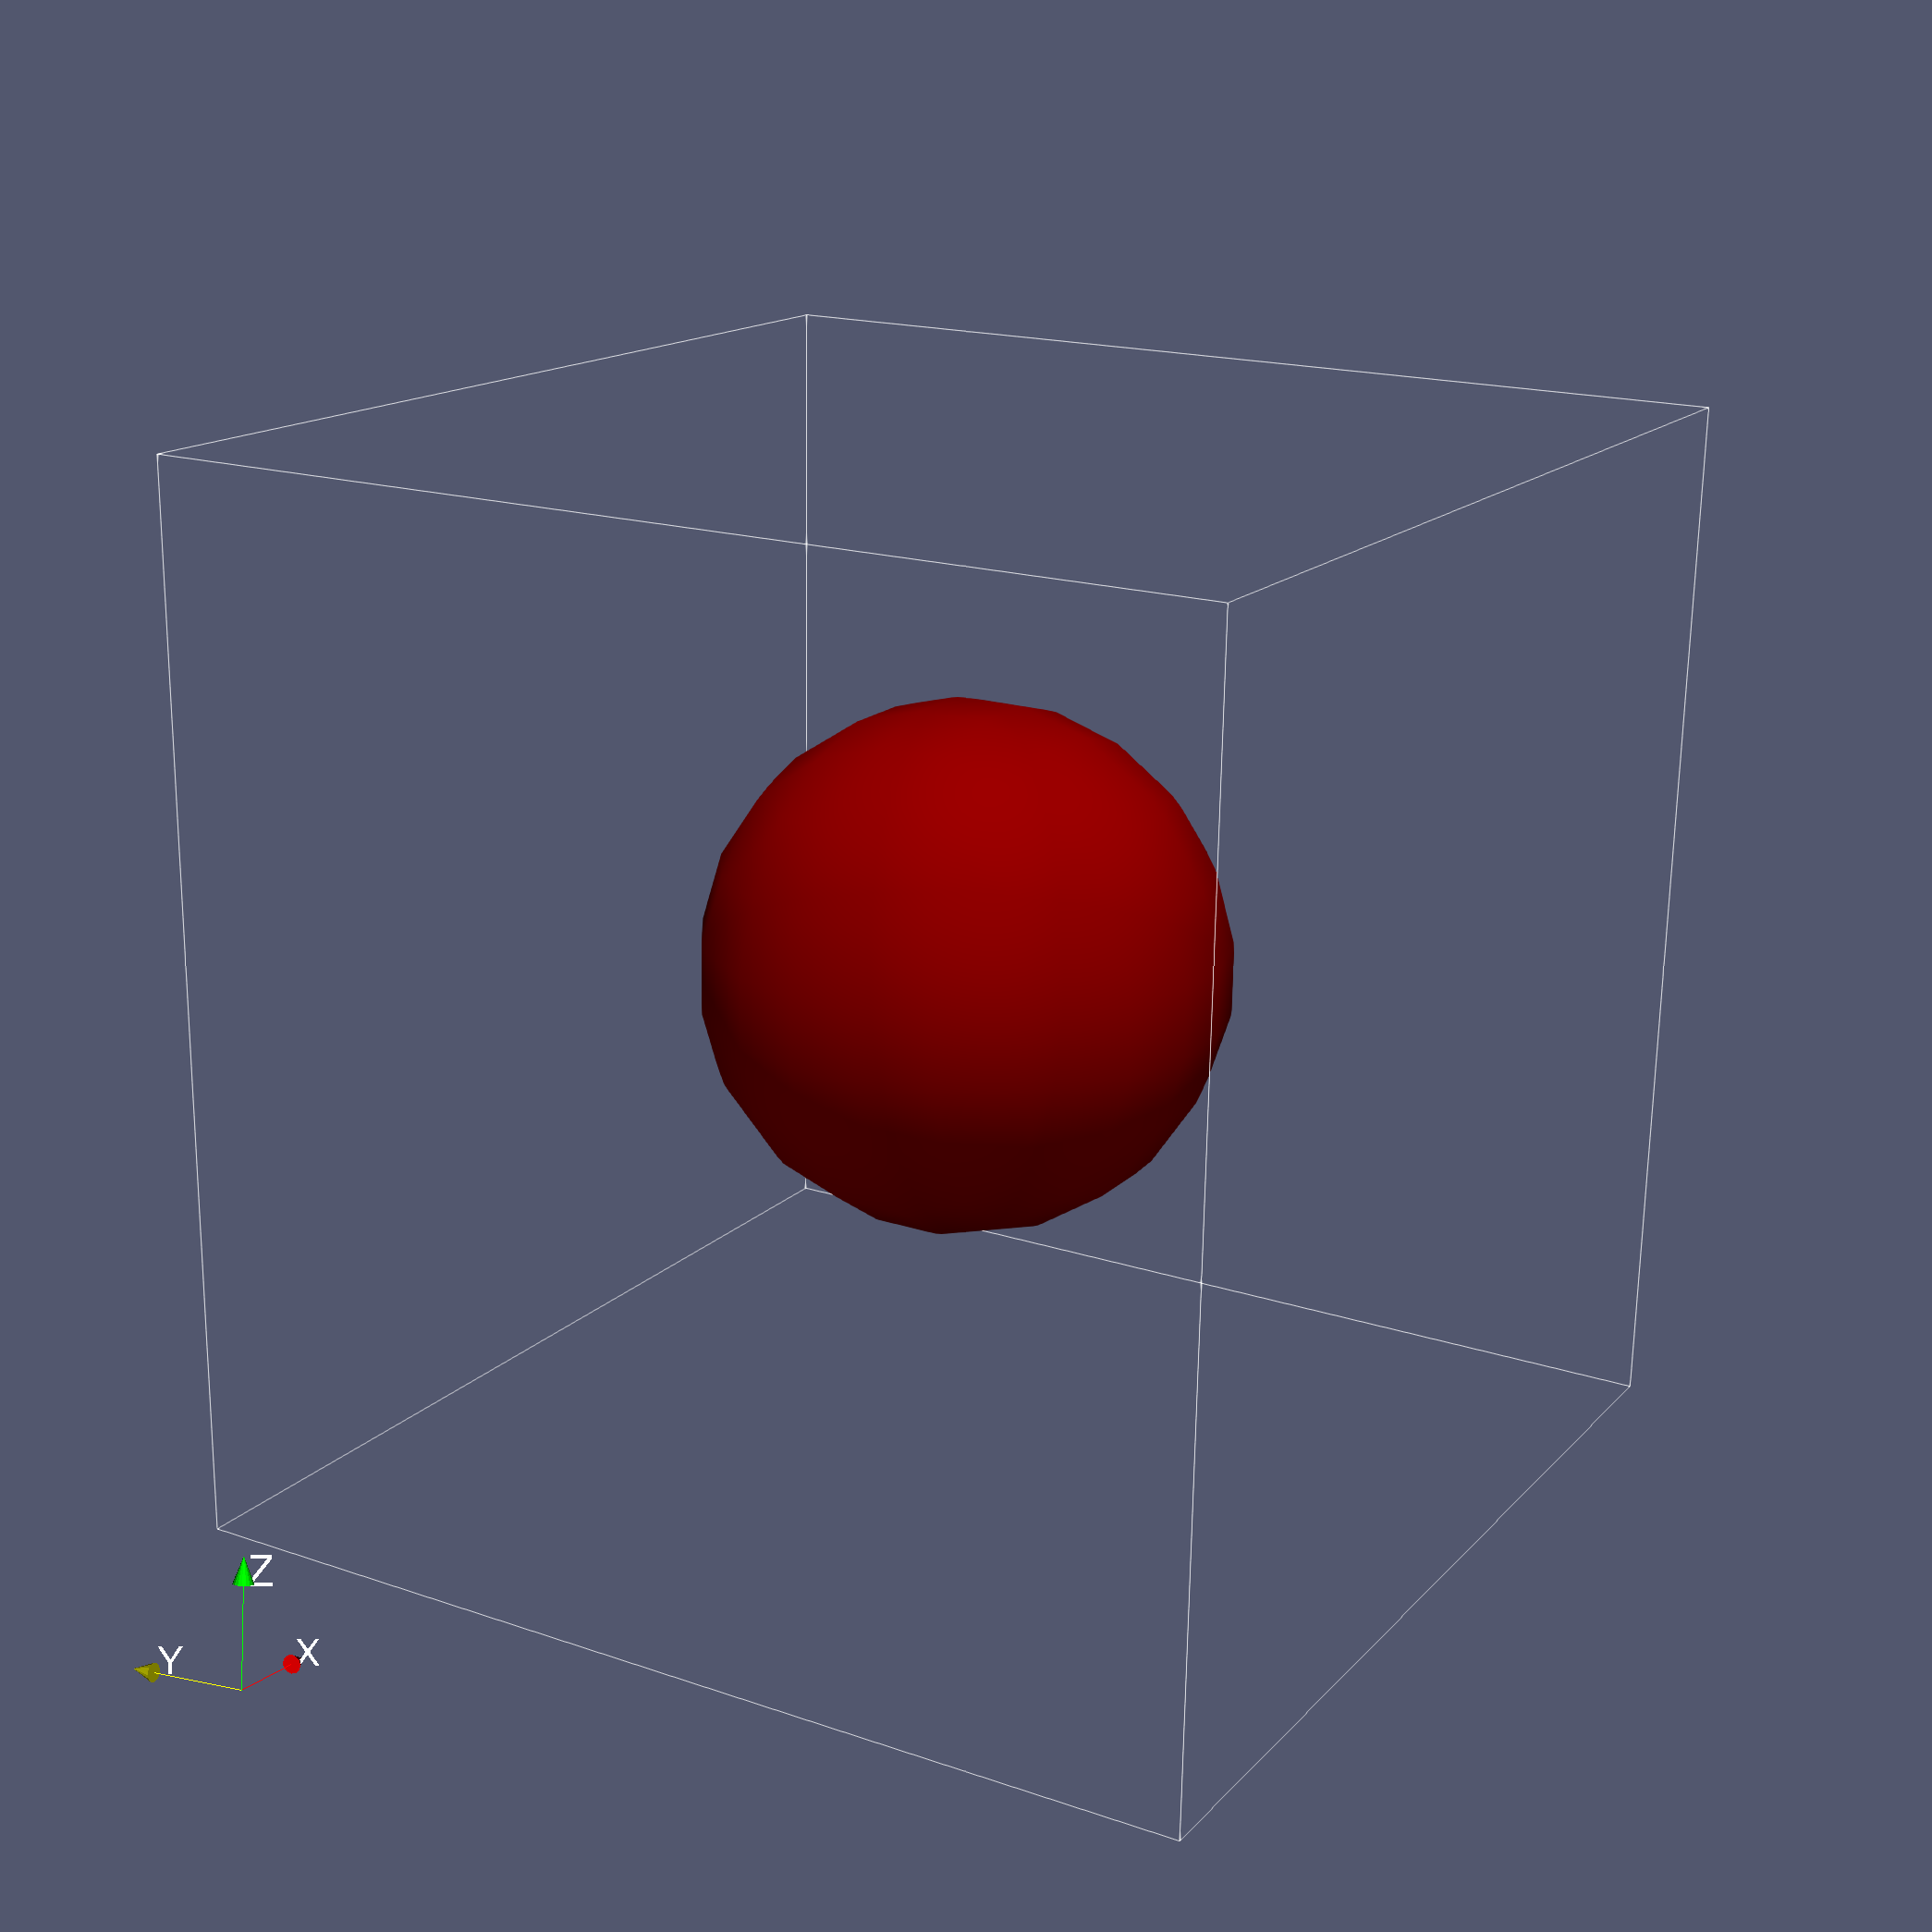
\includegraphics[width=0.49\linewidth]{./figures/sphere_shape.png}
	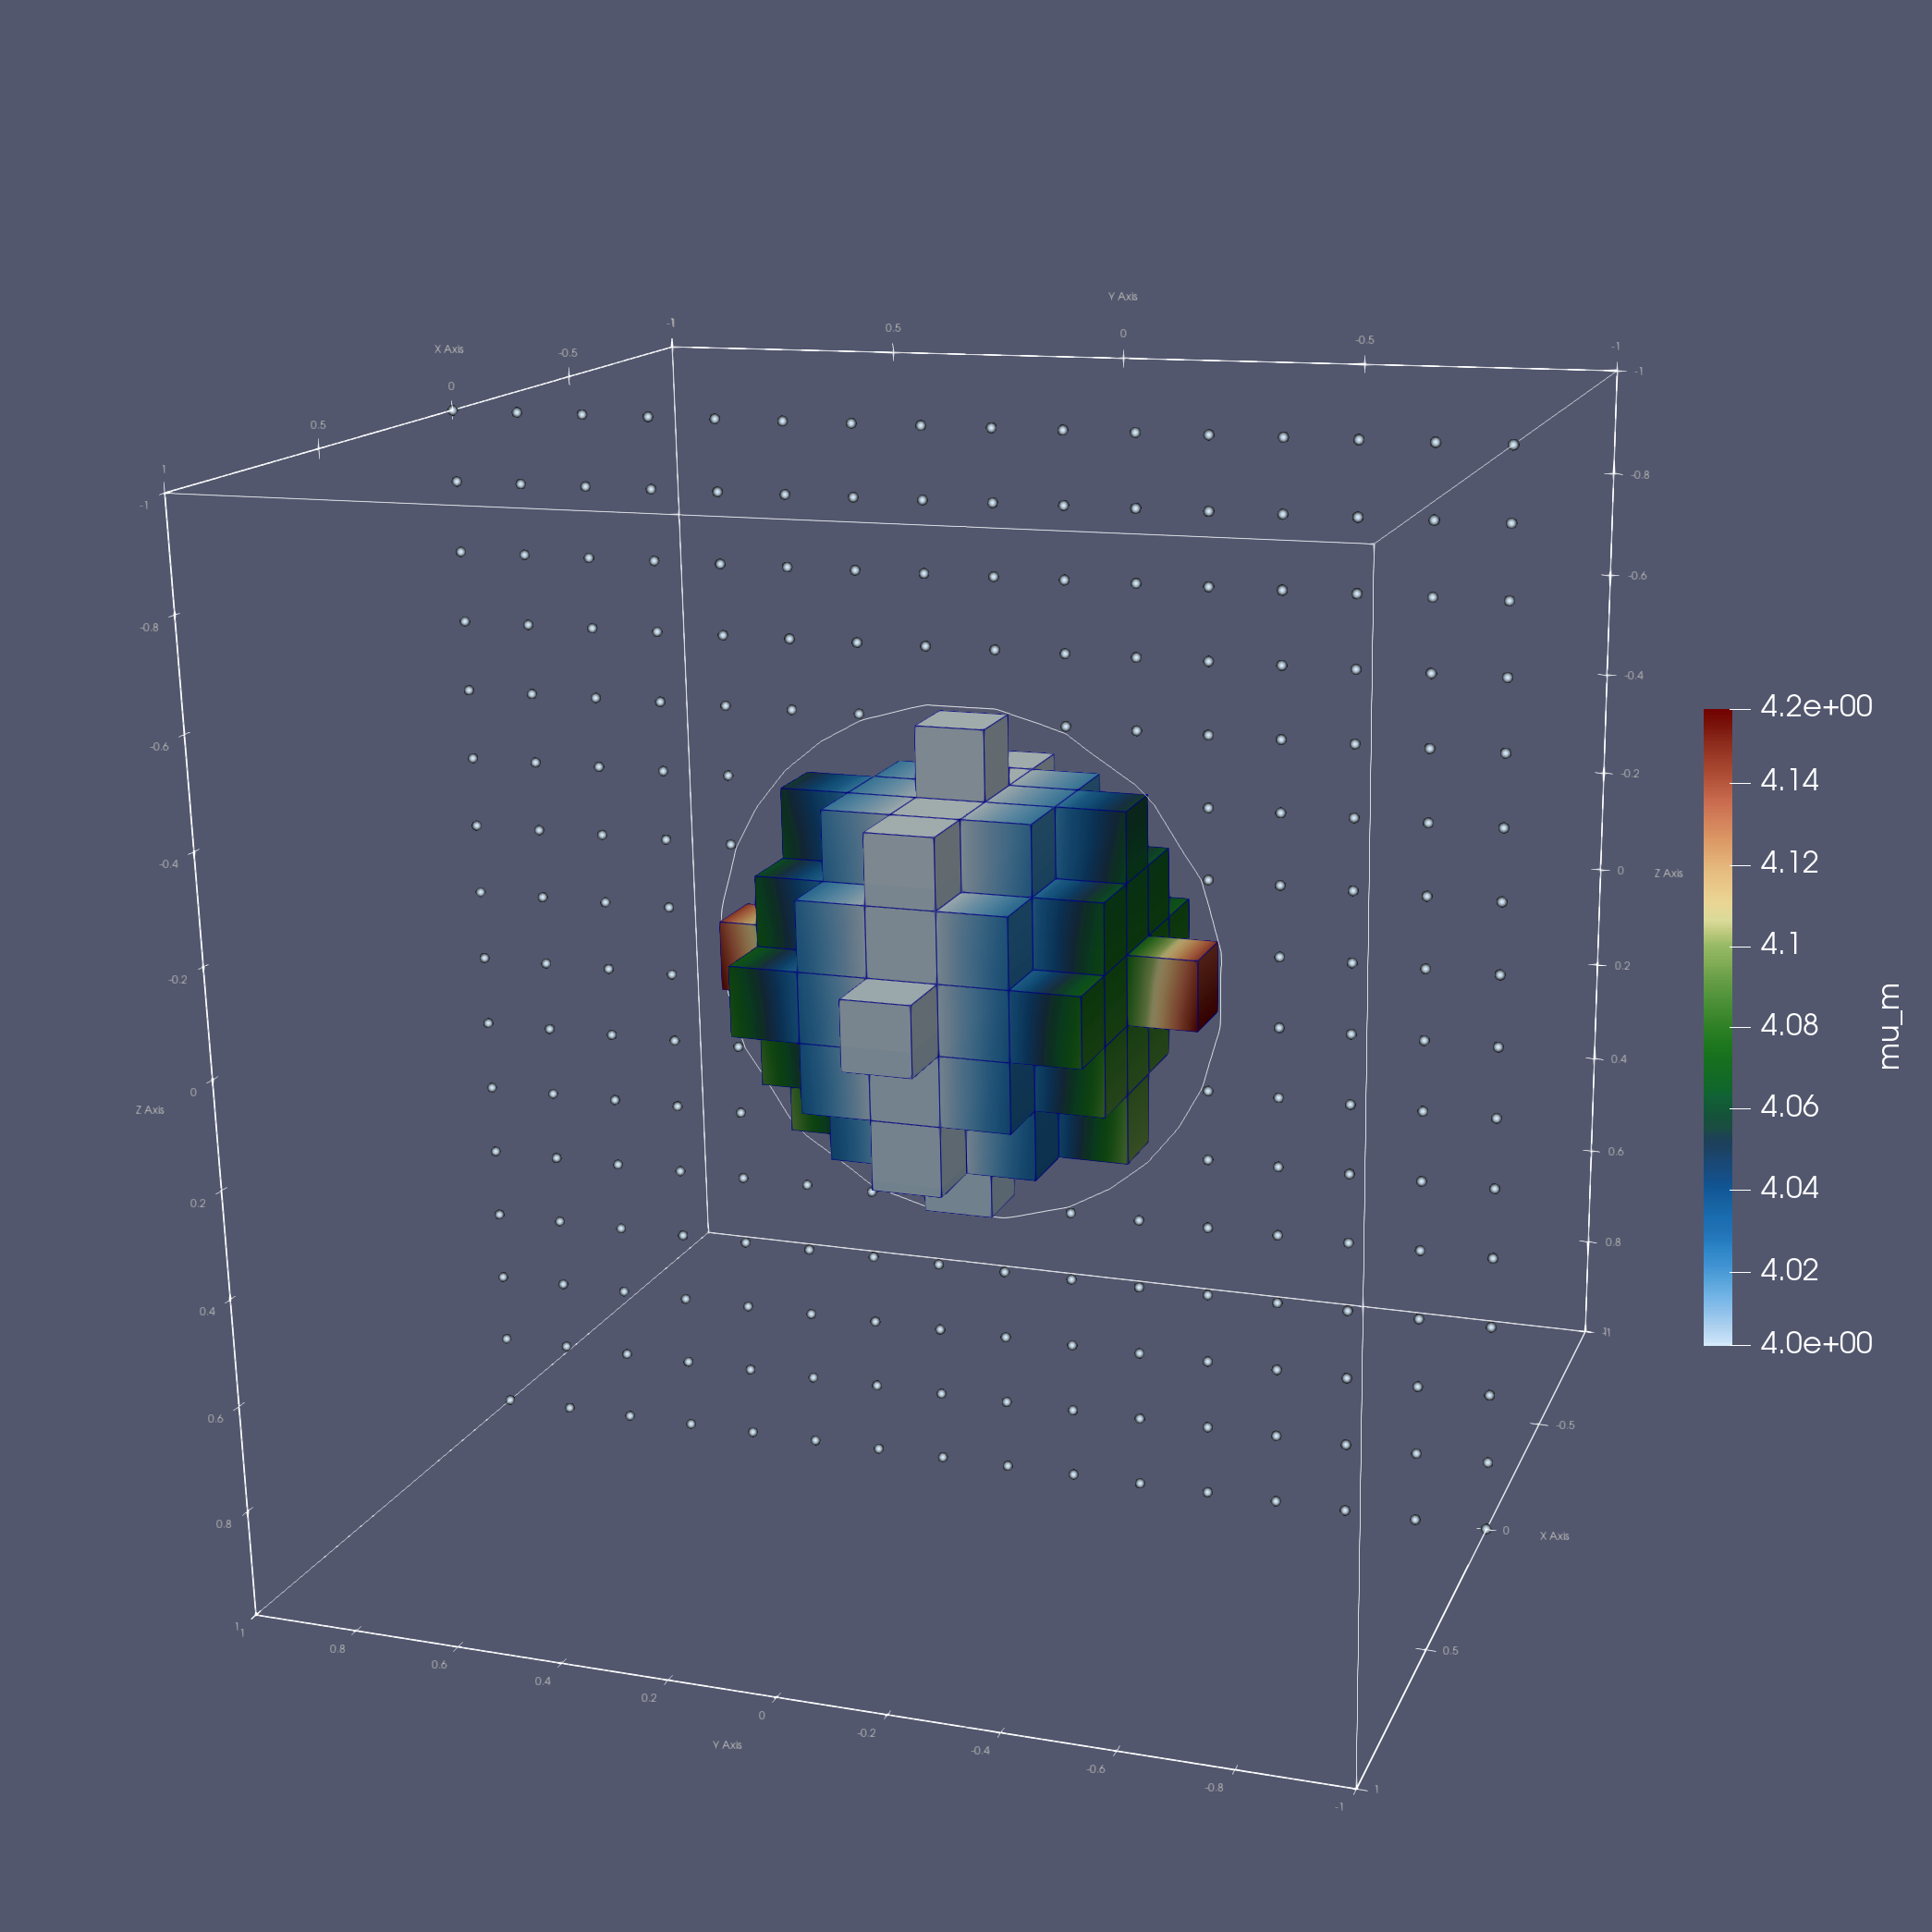
\includegraphics[width=0.49\linewidth]{./figures/sphere_mu_m.png}
	\caption{Illustration of three dimensional interface used (left), and $\mu^\pm$ on the $16\times 16\times 16$ grid (right).}
	\label{fig:sphere}
\end{figure}

\begin{figure}
	\centering
	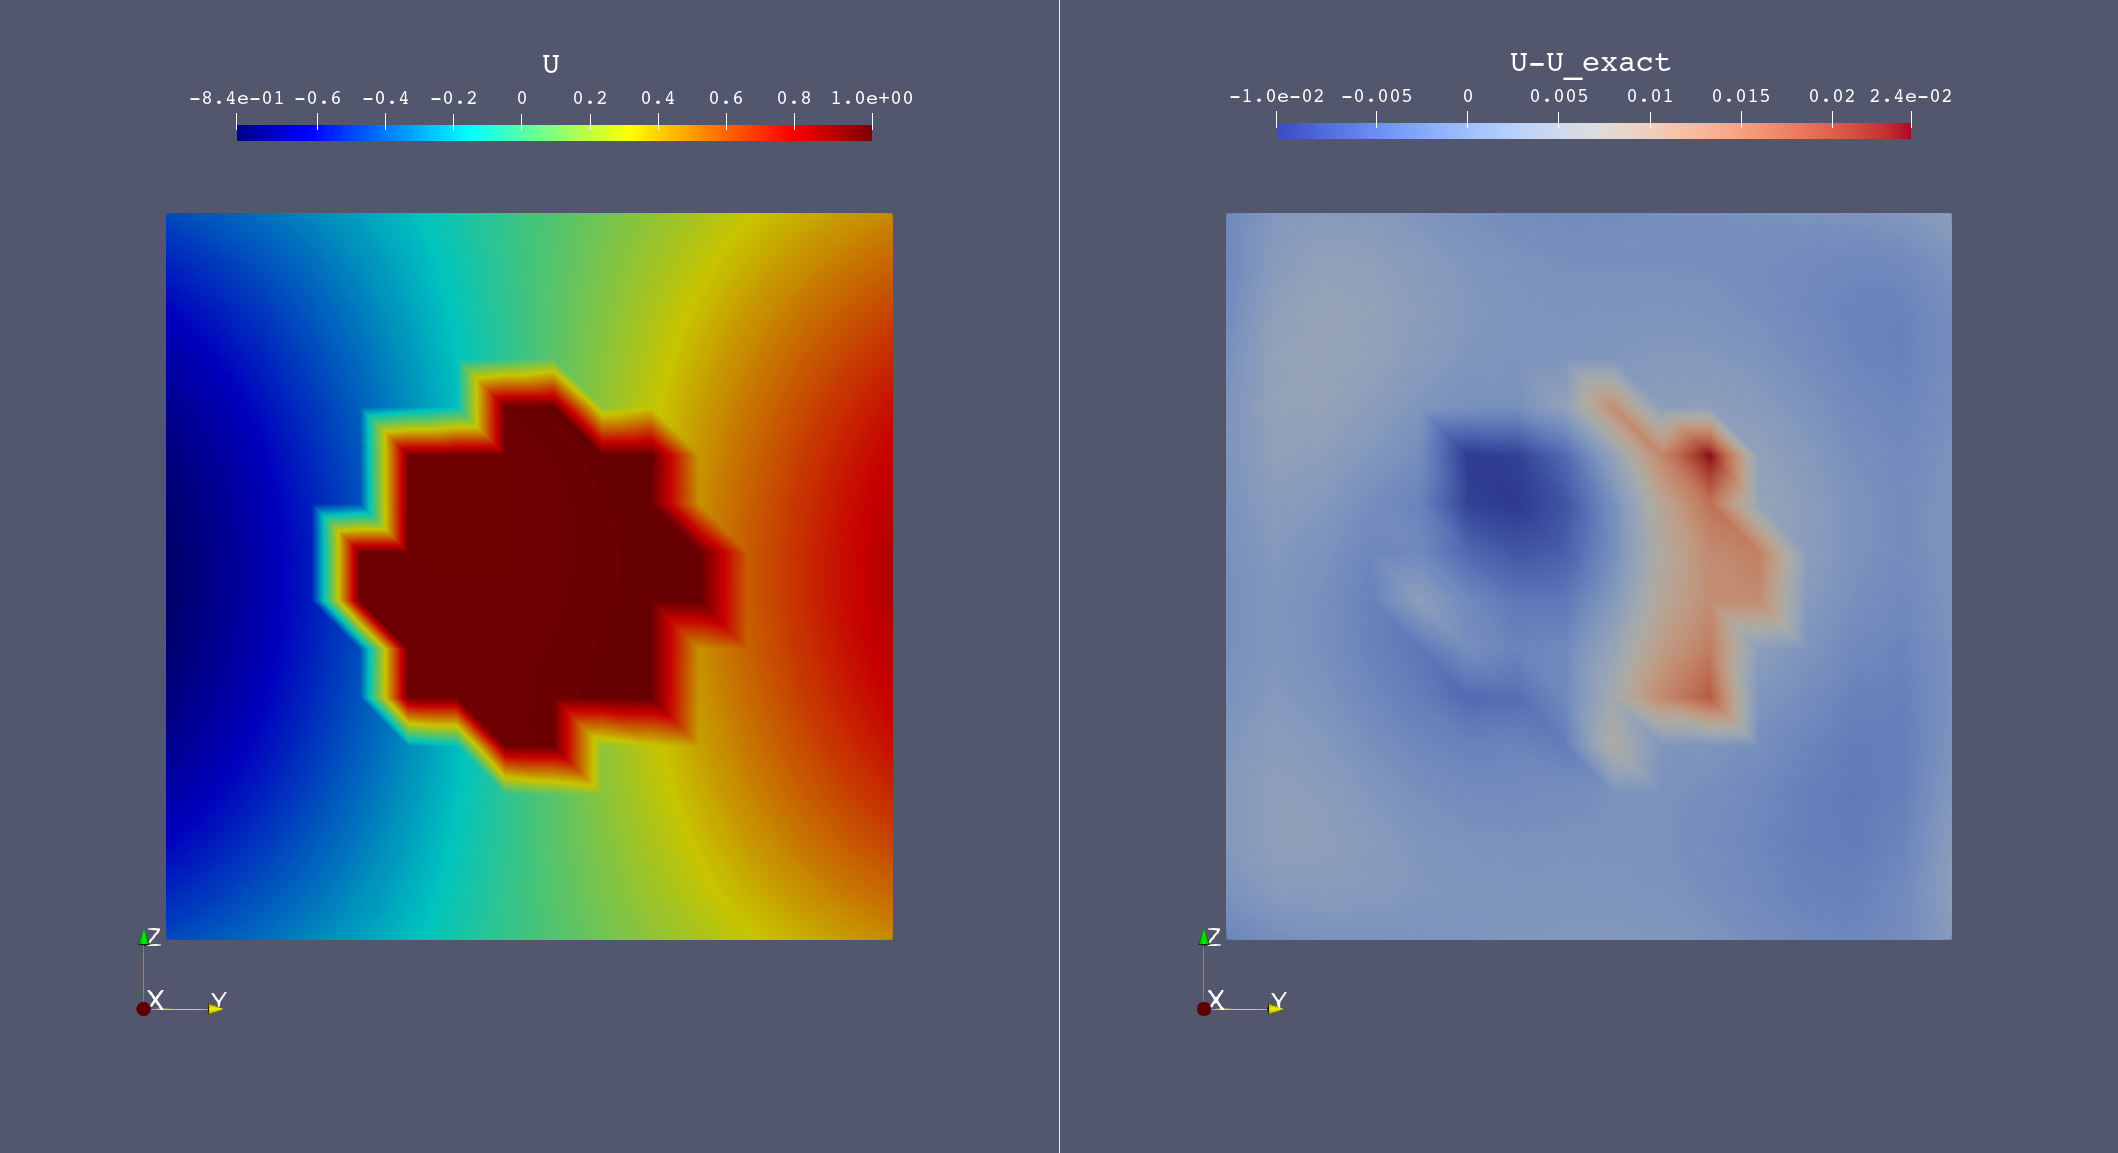
\includegraphics[width=\linewidth]{./figures/sphere_sols_regression_16x16x16.png}
	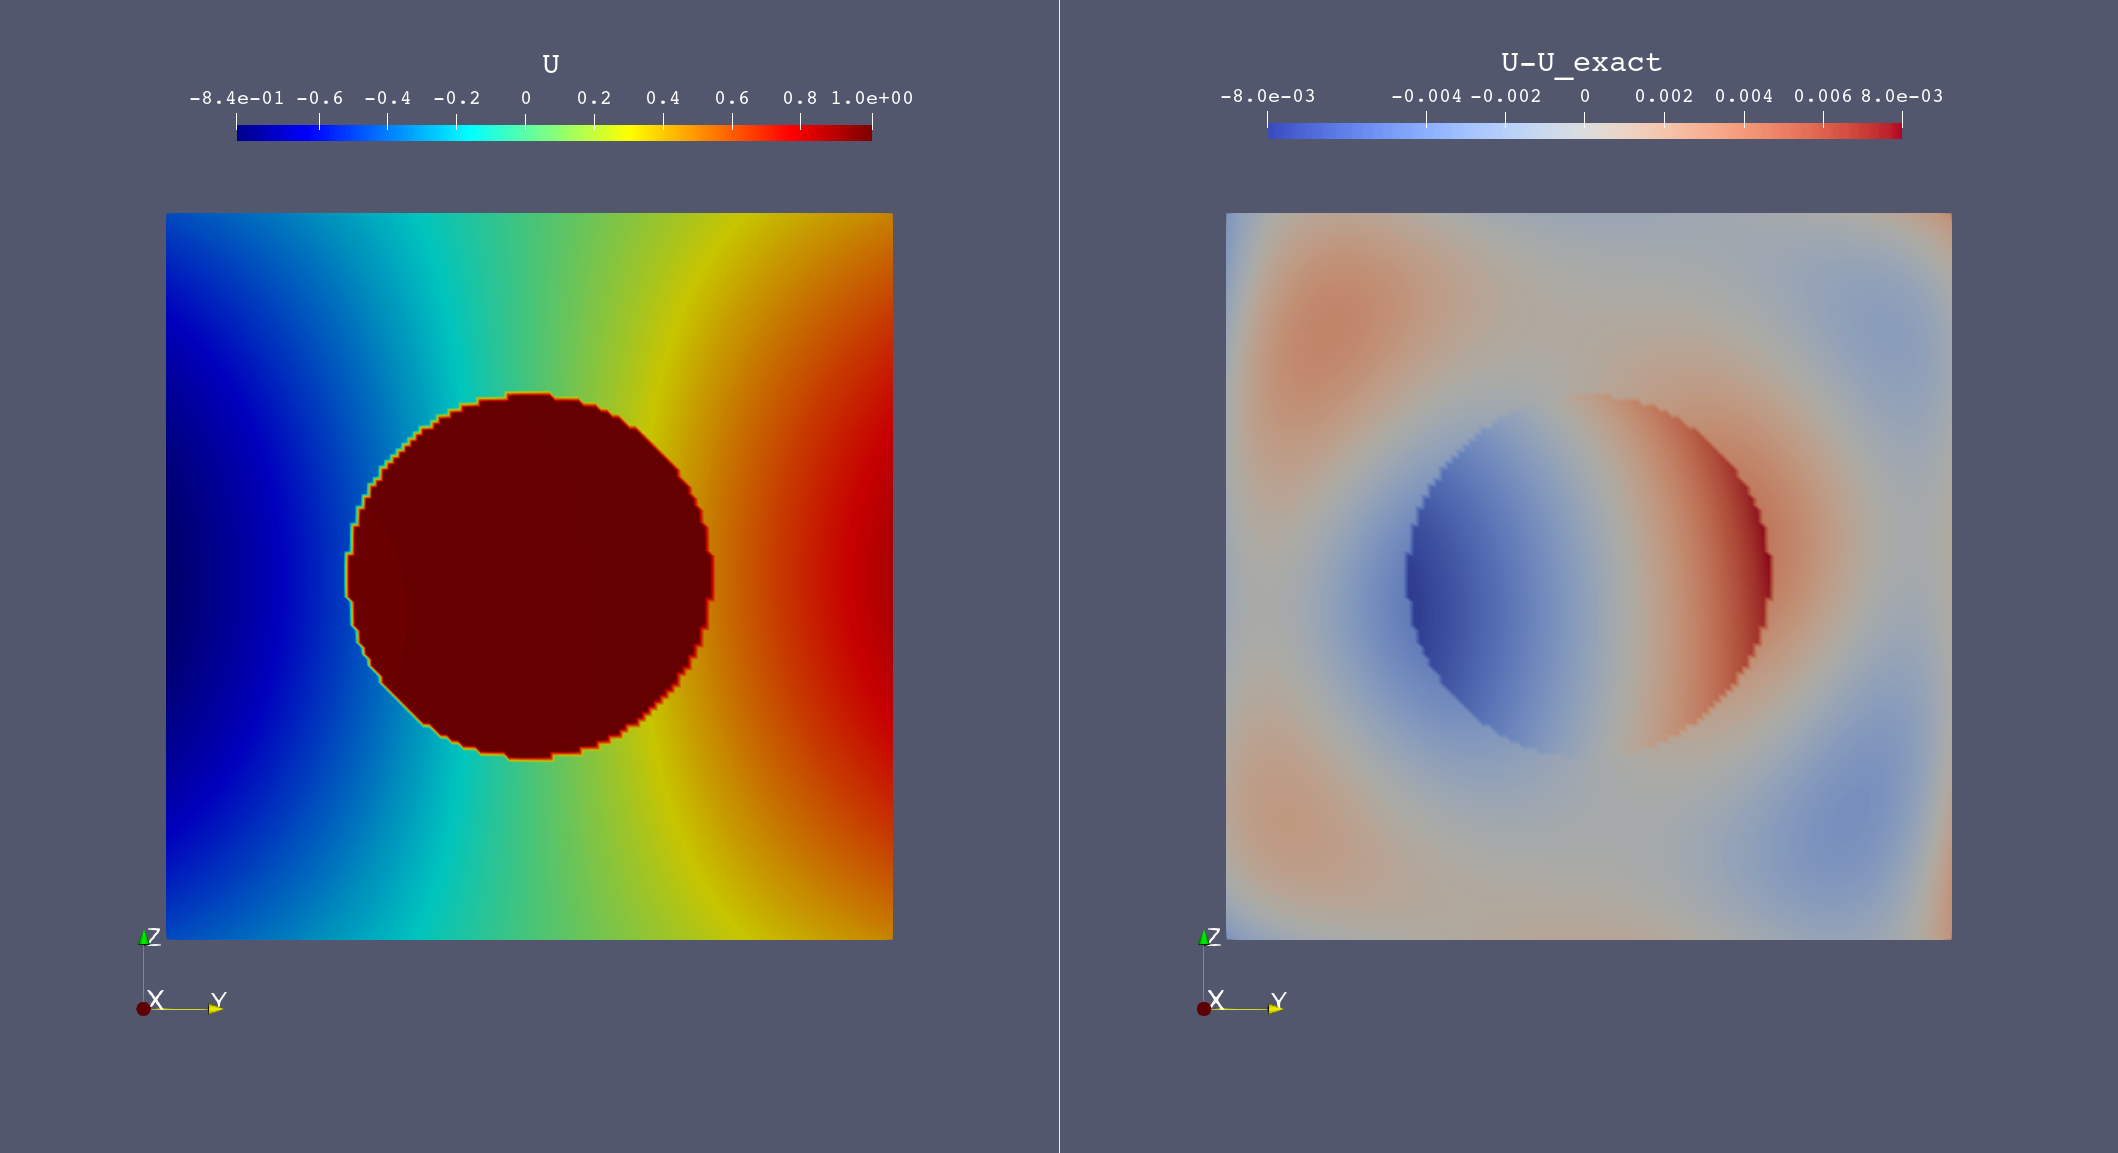
\includegraphics[width=\linewidth]{./figures/sphere_sols_regression_128x128x128.png}
	\caption{Illustration of numerical solution and absolute error using the regression based solver on a cross section of the domain. }
	\label{fig:sphere}
\end{figure}


\begin{figure}
	\centering
	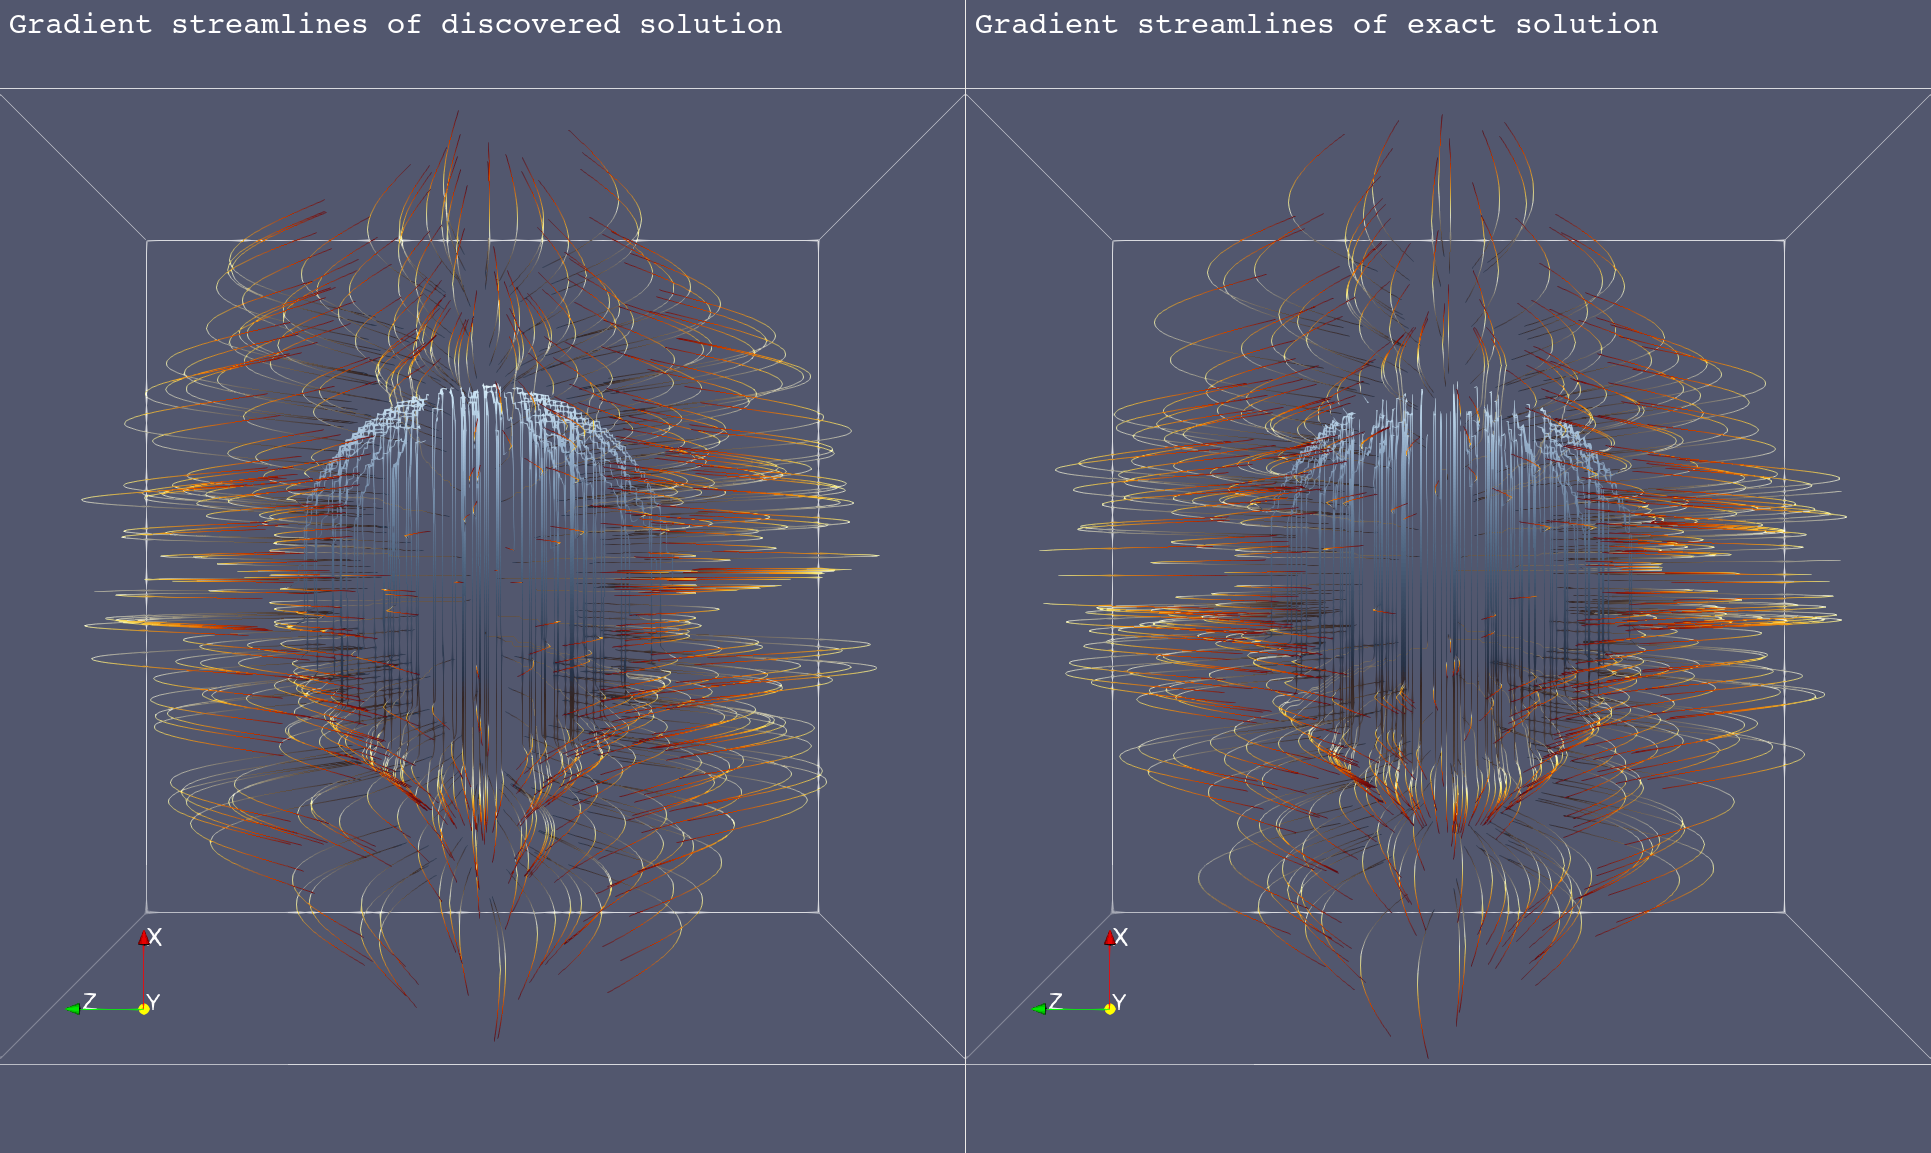
\includegraphics[width=\linewidth]{./figures/128x128x128_electric_U.png}
	\caption{Streamlines of solution gradient for (left) the surrogate neural model colored by model solution value, (right) exact streamlines colored by exact solution values.  }
	\label{fig:spheregrad}
\end{figure}


\subsection{Case II.}

We use a pair of fully connected feedforward neural networks, each composed of $1$ hidden layer and $100$ neurons with \texttt{sine} activation function, followed  by an output layer with $1$ linear neuron. There are a total of $1,002$ trainable parameters in the model.

We consider a star-shaped interface with inner and outer radii $r_i=0.151$ and $r_e=0.911$ that is immersed in a box $\Omega:[-1,1]^3$ described by the level-set function

\begin{align*}
\phi(\mathbf{x}) = \sqrt{x^2 + y^2 + z^2} - r_0 \bigg( 1 + \big( \frac{x^2 + y^2}{x^2 + y^2 + z^2}\big)^2  \sum_{k=1}^3 \beta_k \cos\big(n_k \big(\arctan\big(\frac{y}{x}\big) - \theta_k\big) \big) \bigg)
\end{align*}
with the parameters
\begin{align*}
&r_0 = 0.483, &\begin{pmatrix}
n_1\\
\beta_1\\
\theta_1
\end{pmatrix}=\begin{pmatrix}
3\\
0.1\\
0.5
\end{pmatrix}, &\begin{pmatrix}
n_2\\
\beta_2\\
\theta_2
\end{pmatrix}=\begin{pmatrix}
4\\
-0.1\\
1.8
\end{pmatrix}, &\begin{pmatrix}
n_3\\
\beta_3\\
\theta_3
\end{pmatrix}=\begin{pmatrix}
7\\
0.15\\
0
\end{pmatrix}
\end{align*}

Considering an exact solution 
\begin{align*}
& u^-(x,y,z)=\sin(2x)\cos(2y) e^{z}, & \phi(\mathbf{x})<0\\
& u^+(x,y,z)=\bigg[ 16\big(\frac{y-x}{3}\big)^5 - 20 \big(\frac{y-x}{3}\big)^3 + 5\big( \frac{y-x}{3}\big) \bigg]\ln(x+y+3)\cos(z)          , & \phi(\mathbf{x})\ge 0
\end{align*}
and the diffusion coefficient
\begin{align*}
\mu^-(x,y,z)&=10\bigg[ 1+0.2\cos(2\pi(x+y))\sin(2\pi(x-y)) \cos(z) \bigg] &\phi(\mathbf{x})<0 \\
\mu^+(x,y,z)&=1 &\phi(\mathbf{x})\ge 0 
\end{align*}


\begin{table}[ht]
\begin{center}
\begin{tabular}{|l||ll|ll|c|c|}
\hline
regress $\partial_n$ & \multicolumn{2}{c|}{RMSE}& \multicolumn{2}{c|}{$L^\infty$} & \multicolumn{2}{c|}{GPU Statistics} \\
\hline
$\rm N_{x,y,z}$   &   Solution    &   Order   &   Solution   &   Order & t (sec/epoch) & VRAM (GB)\\
\hline 
$2^3$ & $ 1.36\times 10^{-1}$ &  -     & $ 1.27$   &   -   & $ 0.019  $  & $  0.98 $ \\
$2^4$ & $ 7.98\times 10^{-2} $ &  $ $   & $ 8.23\times 10^{-1} $   & $ $   & $ 0.022  $  & $ 1.01  $ \\ 
$2^5$ & $ 4.36\times 10^{-2} $ &  $ $   & $ 3.85\times 10^{-1} $   & $  $   & $ 0.032  $  & $ 1.30  $ \\ 
$2^6$ & $2.43\times 10^{-2} $ &  $ $   & $ 2.28\times 10^{-1}$   & $ $   & $  0.200 $  & $ 3.7 $ \\ 
$2^7$ & $ $ &  $ $   & $ $   & $ $   & $   $  & $21.4 $ \\ \hline
\end{tabular}
\begin{tabular}{|l||ll|ll|c|c|}
\hline
neural $\partial_n$ & \multicolumn{2}{c|}{RMSE}& \multicolumn{2}{c|}{$L^\infty$} & \multicolumn{2}{c|}{GPU Statistics} \\
\hline
$\rm N_{x,y,z}$   &   Solution    &   Order   &   Solution   &   Order & t (sec/epoch) & VRAM (GB)\\
\hline 
$2^3$ & $2.17\times 10^{-1} $ &  -     & $2.89 $  &   -   & $0.0259 $ & $ 0.93$ \\
$2^4$ & $ 1.34\times 10^{-1	}$ &  $ $   & $ 1.66$  & $ $   & $ 0.0408$ & $1.19 $ \\ 
$2^5$ & $5.68\times 10^{-2} $ &  $ $   & $ 8.17\times 10^{-1}$  & $ $   & $ 0.0712$ & $ 2.96$ \\ 
$2^6$ & $ 2.77\times 10^{-2}$ &  $ $   & $3.94\times 10^{-1} $  & $ $   & $ 0.334 $ & $ 13.6$ \\ 
$2^7$ & OOM  &  -   & OOM  & -   & OOM & OOM \\ \hline
\end{tabular}
\caption{Convergence on the solution using the regression-based solver. We report $L^\infty$-norm error as well as root-mean-squared-error (RMSE) of the solution field evaluated everywhere in the domain. Rightmost column reports the overall time to solution for \texttt{JAX-DIPS} which constitutes $10,000$ epochs in each case and the initial compilation time of jaxpressions. The neural network has $982$ trainable parameters. In each case GPU compute occupancy is at $100\%$ on a single NVIDIA RTX A6000 GPU. The neural network pair have 1 hidden layer each with 100 neurons, overall $1,002$ trainable parameteres. We use a domain switching scheme with the $\textrm{whole region} \rightarrow \textrm{fast region} \rightarrow \textrm{fast region}$ optimization sequence.}
\end{center}
\end{table}





\begin{figure}
	\centering
	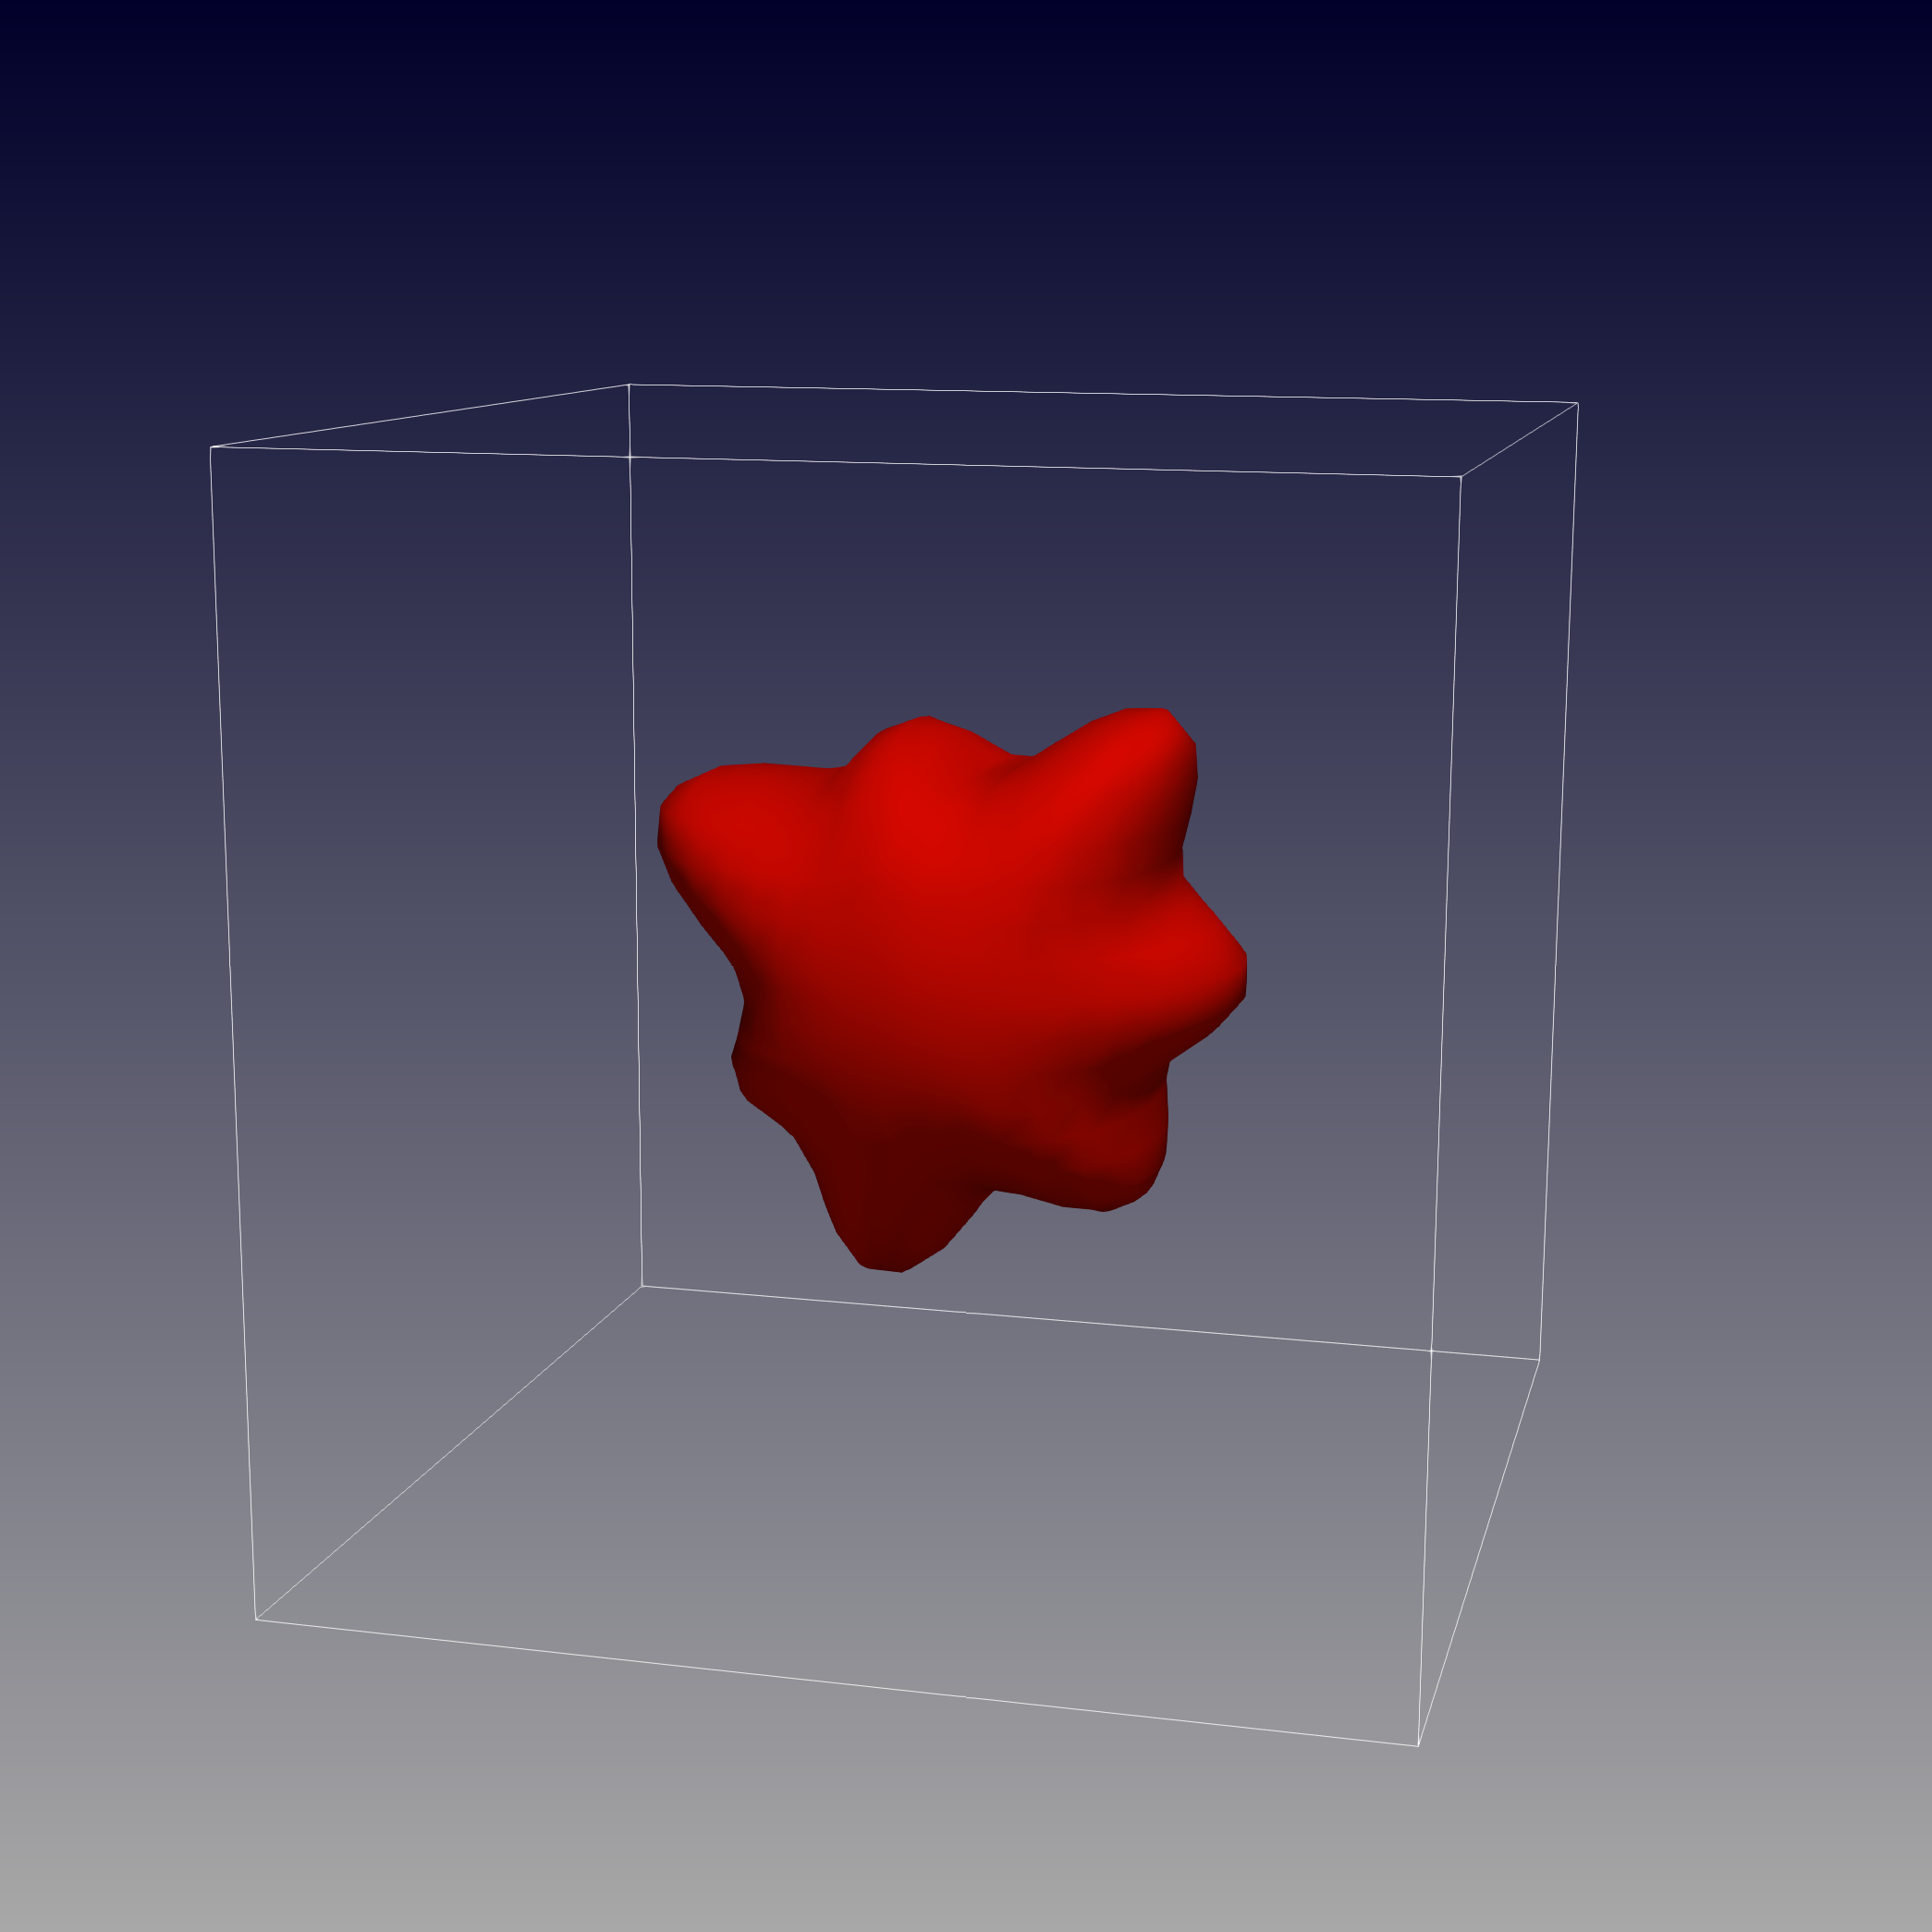
\includegraphics[width=0.49\linewidth]{./figures/star_shape.png}
	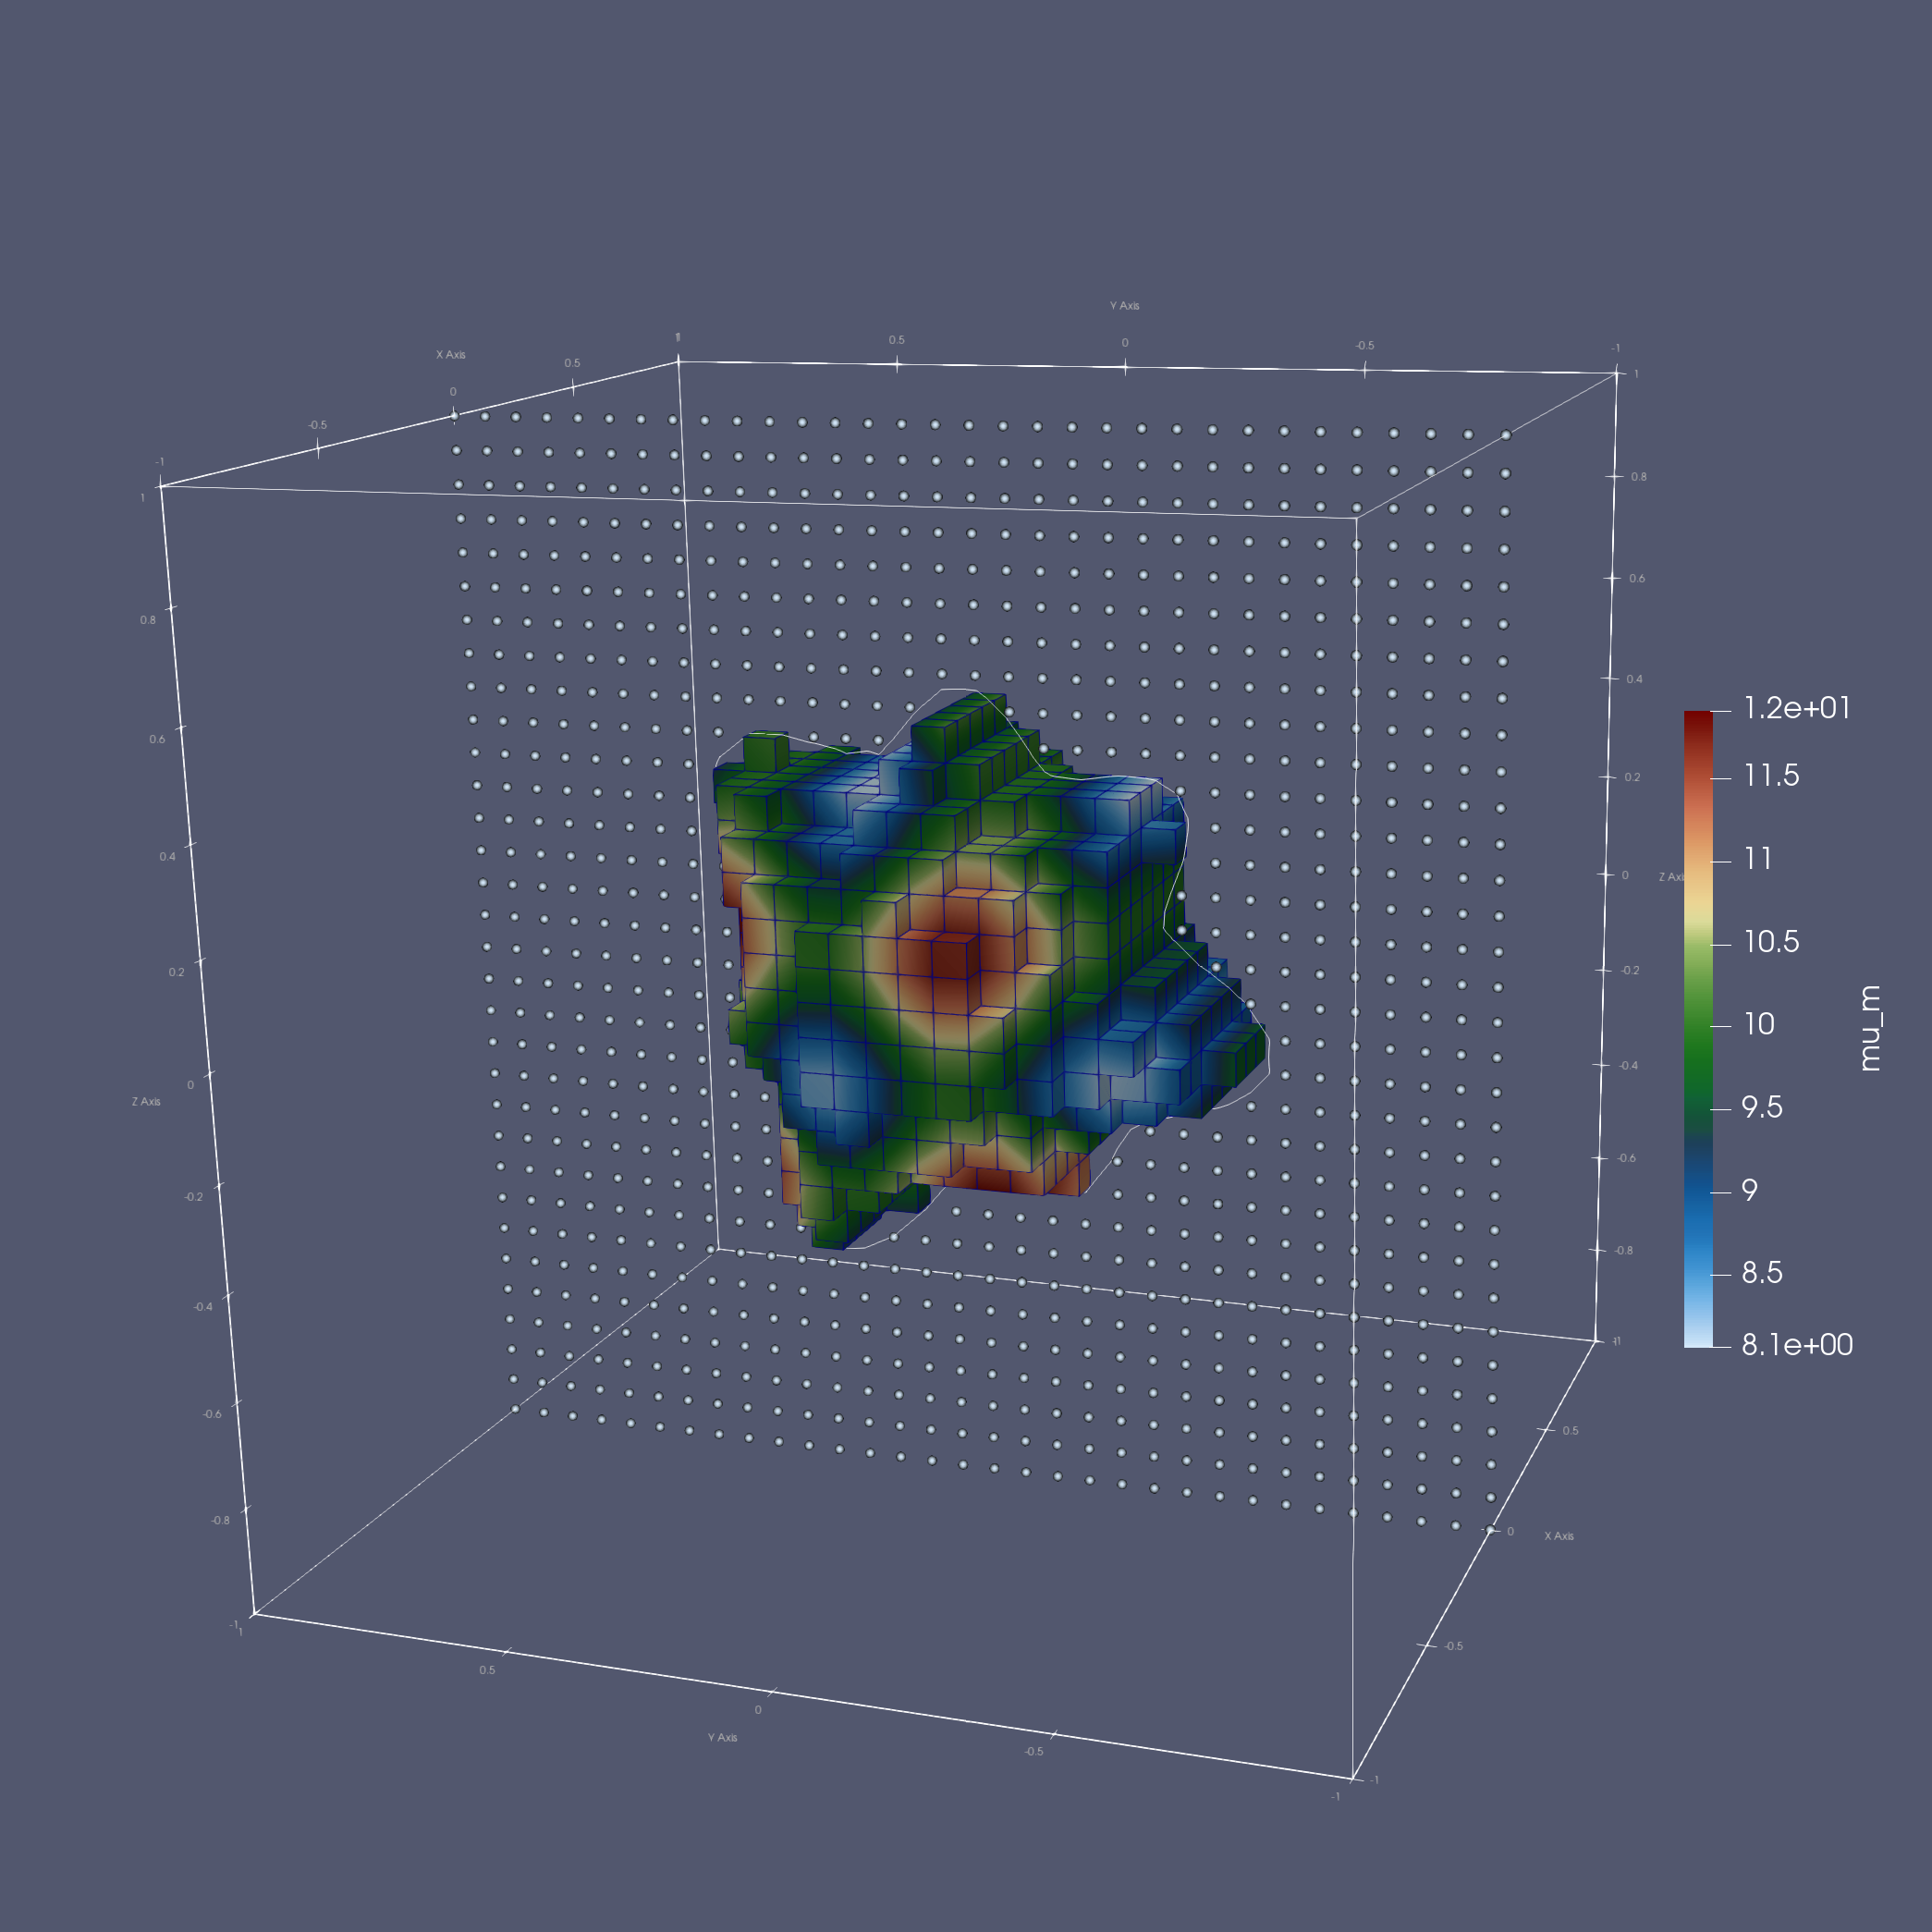
\includegraphics[width=0.49\linewidth]{./figures/star_mu_m.png}
	\caption{Illustration of three dimensional interface used (left), and $\mu^\pm$ on the $32\times 32\times 32$ grid (right).}
	\label{fig:star}
\end{figure}

\begin{figure}
	\centering
	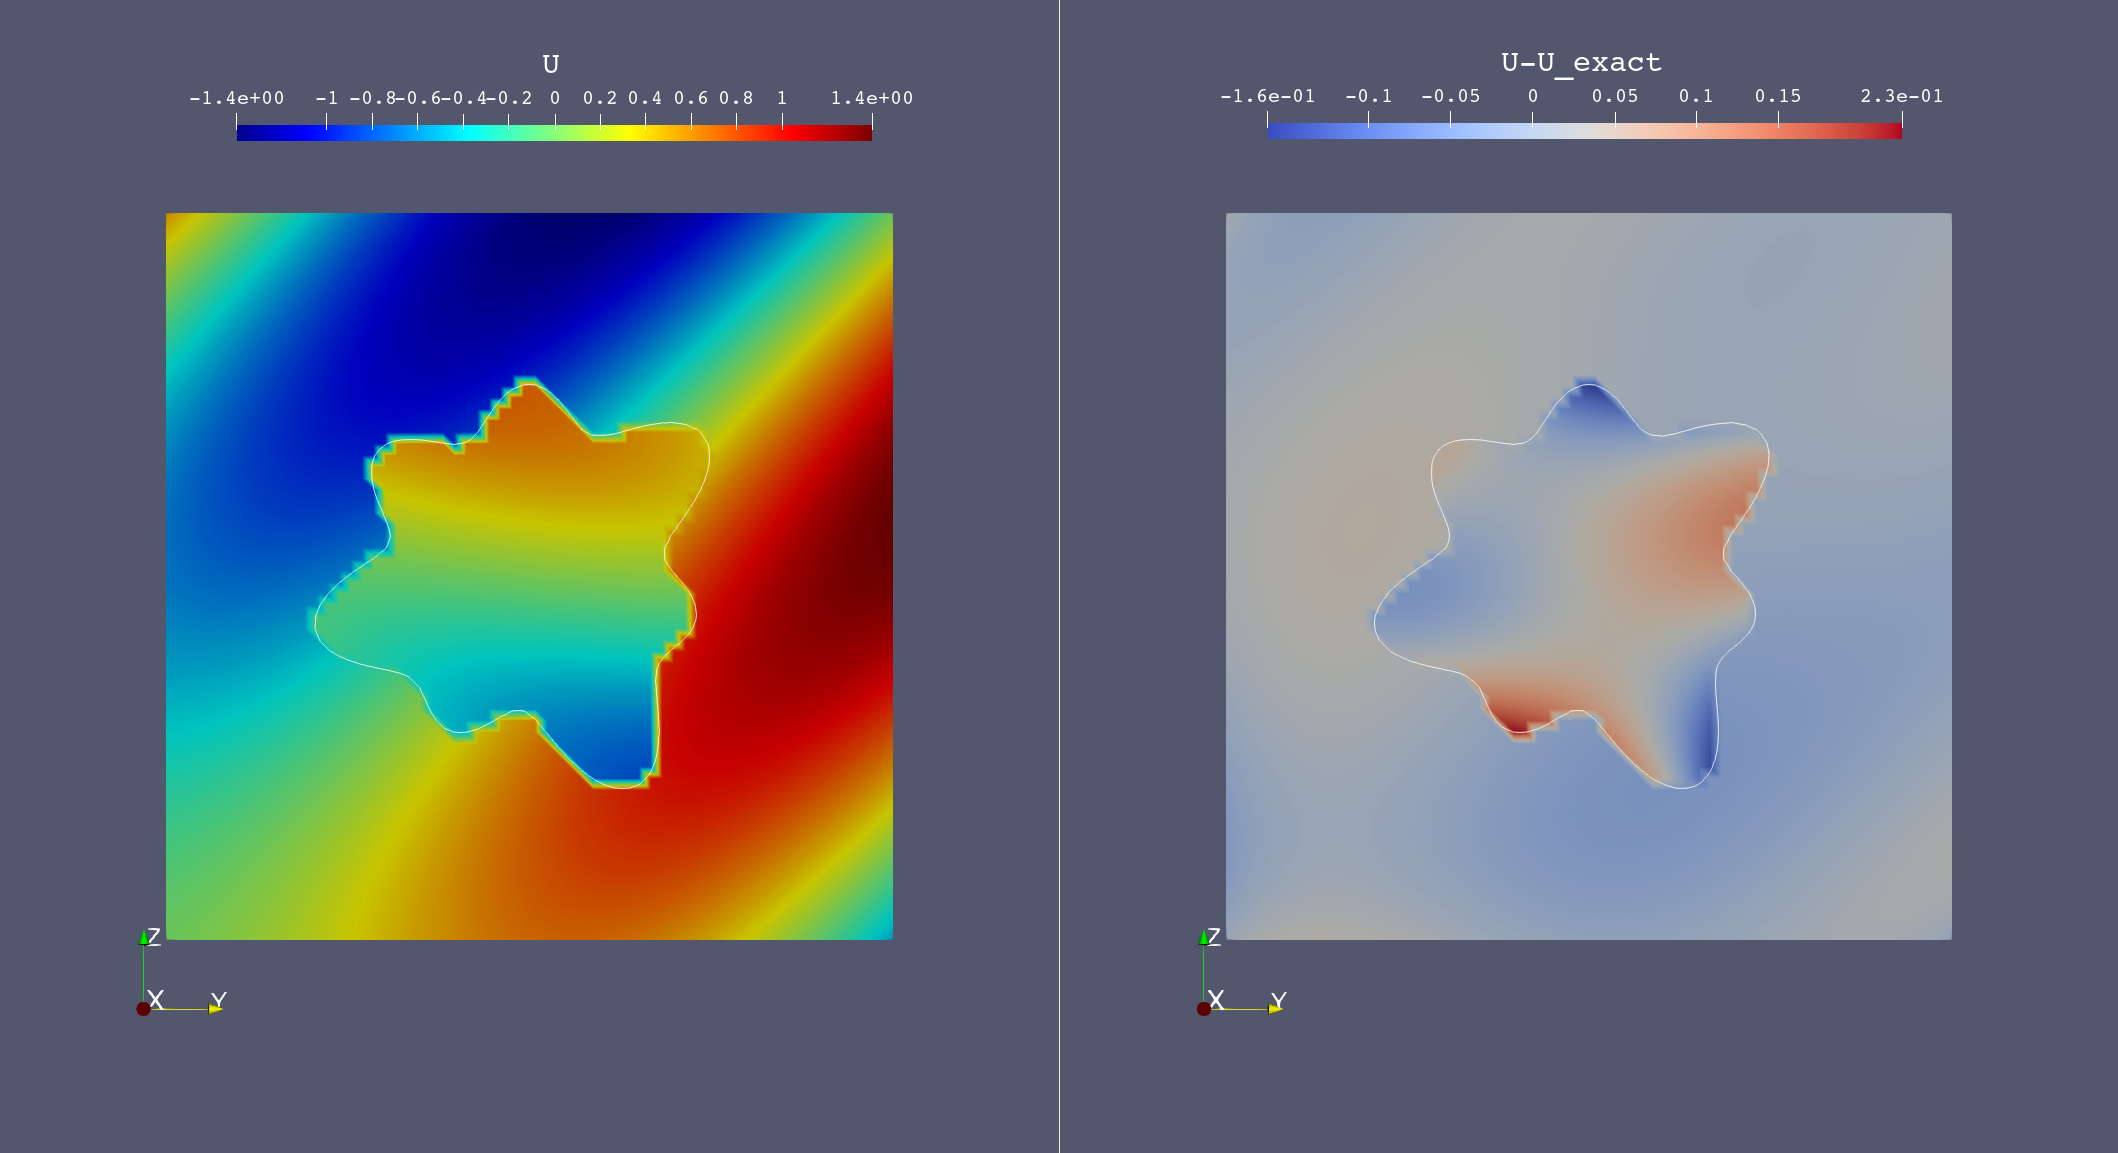
\includegraphics[width=\linewidth]{./figures/star_sols_regression_64x64x64.png}
	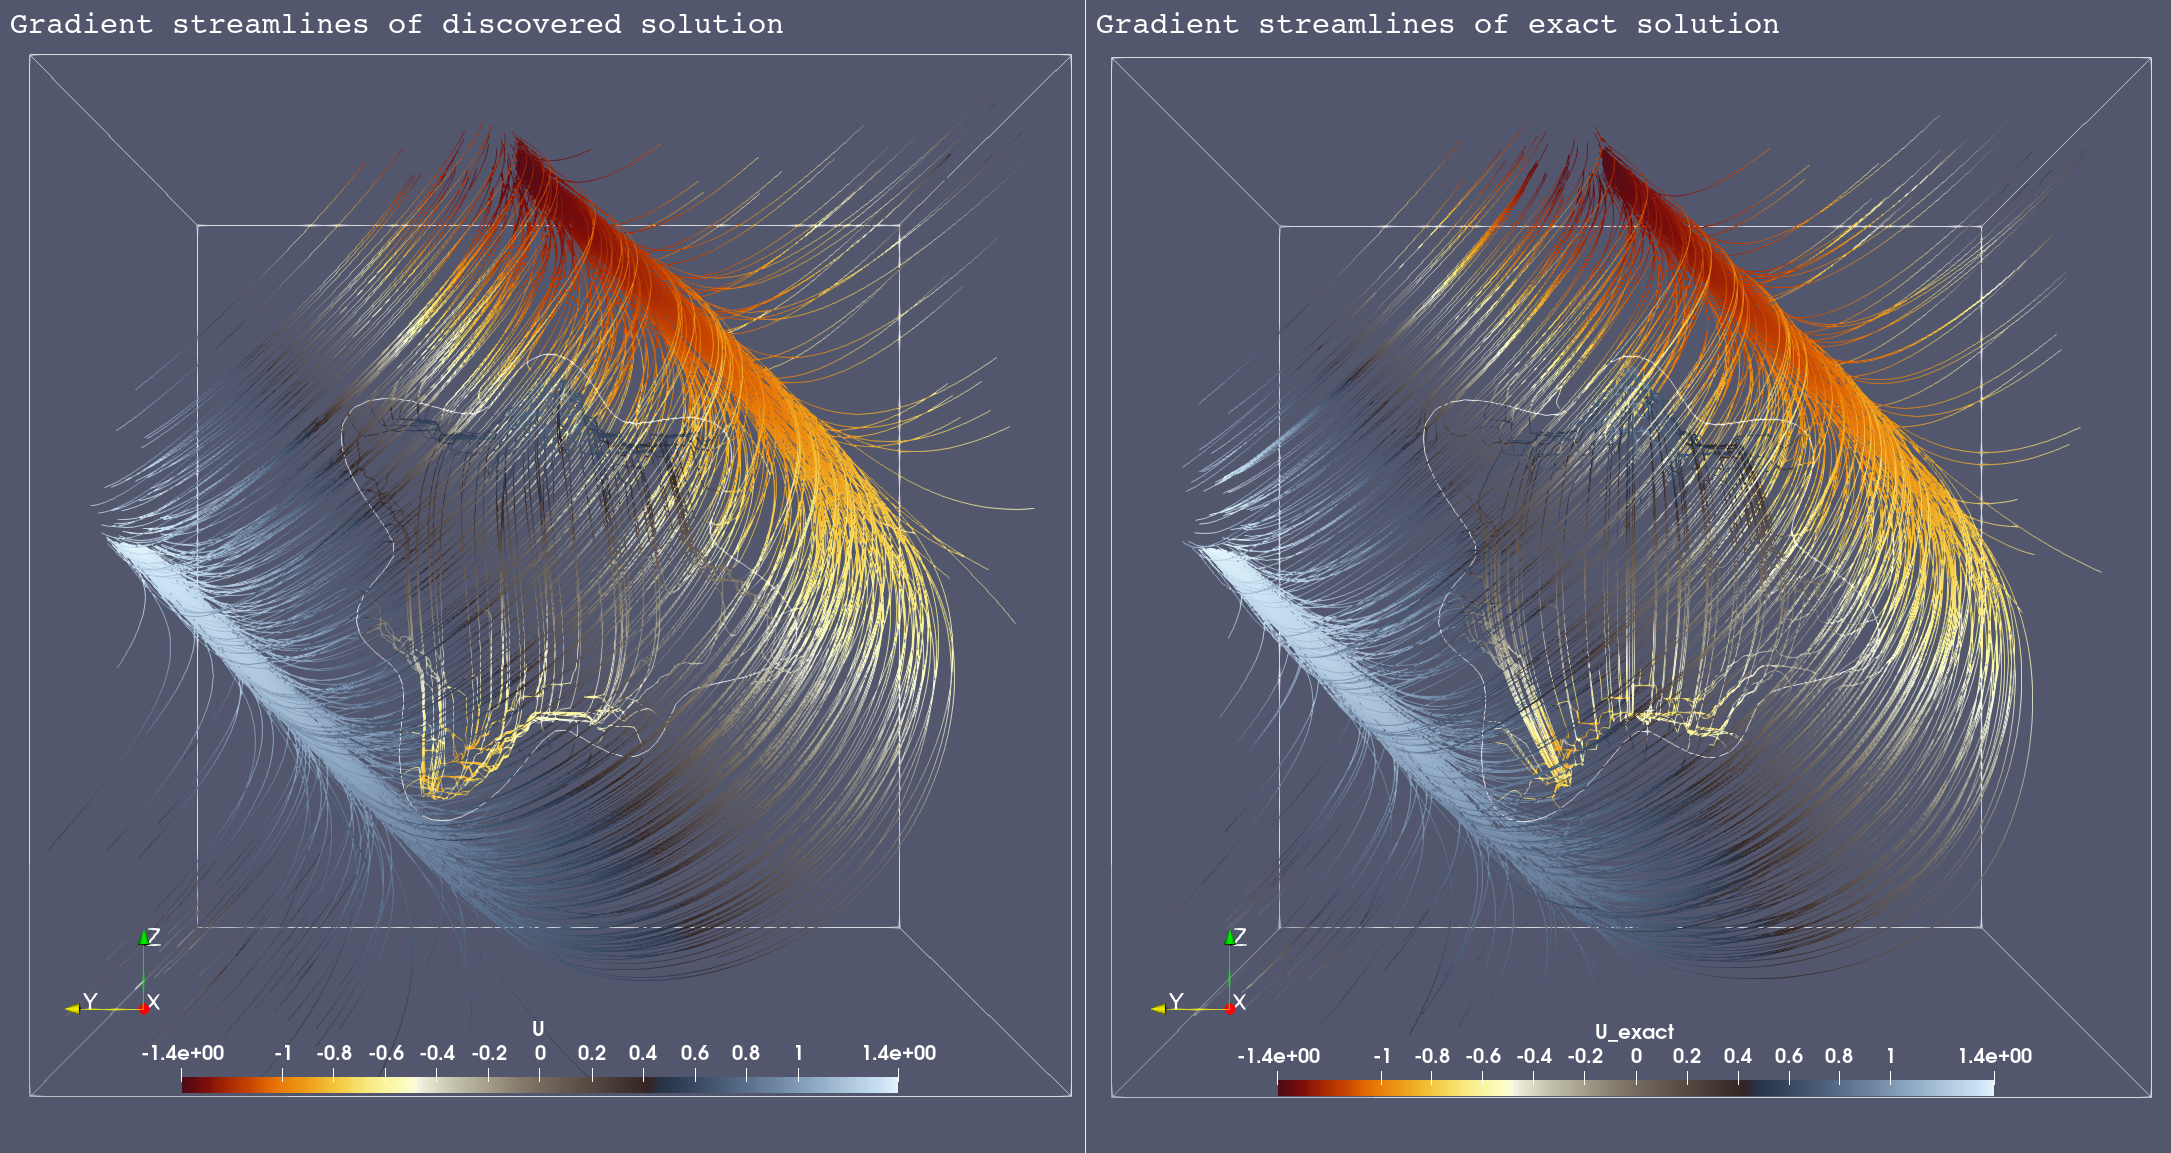
\includegraphics[width=\linewidth]{./figures/star_grad_sols_regression_64x64x64.png}
	\caption{Illustration of exact and numerical solutions on a $64\times 64 \times 64$ grid.}
	\label{fig:star_sol}
\end{figure}


\begin{figure}
	\centering
	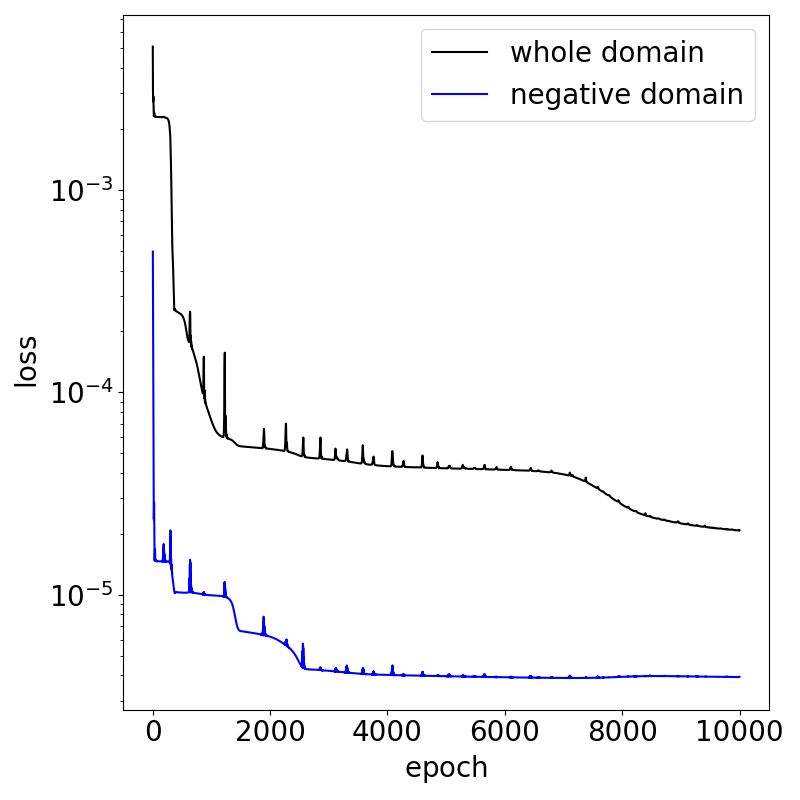
\includegraphics[width=0.49\linewidth]{./figures/poisson_solver_loss_star_64x64x64_regress.png}
	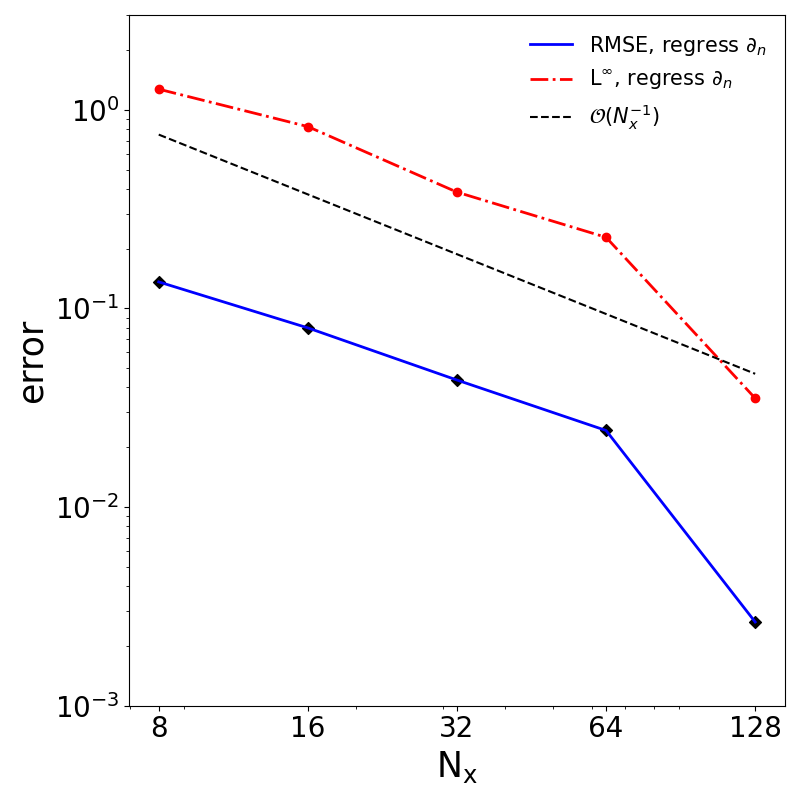
\includegraphics[width=0.45\linewidth]{./figures/case_II_regression.png}
	\caption{Loss evolution with epochs for the sphere of $64\times 64\times 64$ grid (left) and different accuracy measures at 5 resolutions (right).}
	\label{fig:lossestar}
\end{figure}

\section{Conclusion \& Future Directions}
We developed a differentiable GPU-based framework for solving partial differential equations with jump conditions across irregular interfaces in three spatial dimensions. Solutions in each domain are represented by a simple multi-layer perceptron (MLP) and Cartesian grid points of the underlying numerical discretization scheme are treated as collocation points for optimizing the unknown parameters of the MLPs. 


There are many improvements for \texttt{JAX-DIPS} that we will pursue for future development:

\begin{itemize}

\item  More sophisticated neural architectures can be considered in \texttt{JAX-DIPS} by adding to the model class of the library. We only considered MLPs, however in recent years there have a plethora of deep neural network models that have shown great promise such as transformers, graph neural networks, \textit{etc}.

\item Multi-GPU training using domain decomposition and distribution using the \texttt{pmap} primitive in JAX is another very immediate improvement that will enable higher resolution simulations.

\item Modification of the numerical discretization scheme in order to operate over unstructured point clouds rather than the uniform Cartesian grids.

\item Extension to adaptive grids with enhanced resolutions closer to the interfaces while coarsening the grid cells in the bulk.


\end{itemize}

\section*{Acknowledgement}



%%%%%%%%%%%
\newpage
%\section*{References}
\bibliographystyle{abbrv}
\addcontentsline{toc}{section}{\refname}
\bibliography{references}

\end{document}
